%% abtex2-modelo-relatorio-tecnico.tex, v-1.9.7 laurocesar
%% Copyright 2012-2018 by abnTeX2 group at http://www.abntex.net.br/ 
%%
%% This work may be distributed and/or modified under the
%% conditions of the LaTeX Project Public License, either version 1.3
%% of this license or (at your option) any later version.
%% The latest version of this license is in
%%   http://www.latex-project.org/lppl.txt
%% and version 1.3 or later is part of all distributions of LaTeX
%% version 2005/12/01 or later.
%%
%% This work has the LPPL maintenance status `maintained'.
%% 
%% The Current Maintainer of this work is the abnTeX2 team, led
%% by Lauro César Araujo. Further information are available on 
%% http://www.abntex.net.br/
%%
%% This work consists of the files abntex2-modelo-relatorio-tecnico.tex,
%% abntex2-modelo-include-comandos and abntex2-modelo-references.bib
%%

% ------------------------------------------------------------------------
% ------------------------------------------------------------------------
% abnTeX2: Modelo de Relatório Técnico/Acadêmico em conformidade com 
% ABNT NBR 10719:2015 Informação e documentação - Relatório técnico e/ou
% científico - Apresentação
% ------------------------------------------------------------------------ 
% ------------------------------------------------------------------------

\documentclass[
	% -- opções da classe memoir --
	12pt,				% tamanho da fonte
	openany,			% capítulos começam em pág ímpar (insere página vazia caso preciso)
	oneside,			% para impressão em recto e verso. Oposto a oneside
	a4paper,			% tamanho do papel. 
	% -- opções da classe abntex2 --
	%chapter=TITLE,		% títulos de capítulos convertidos em letras maiúsculas
	%section=TITLE,		% títulos de seções convertidos em letras maiúsculas
	%subsection=TITLE,	% títulos de subseções convertidos em letras maiúsculas
	%subsubsection=TITLE,% títulos de subsubseções convertidos em letras maiúsculas
	% -- opções do pacote babel --
	english,			% idioma adicional para hifenização
	french,				% idioma adicional para hifenização
	spanish,			% idioma adicional para hifenização
	brazil,				% o último idioma é o principal do documento
	]{abntex2}

%\documentclass[12pt,a4paper,openany,oneside]{abntex2}
% ---
% PACOTES
% ---

% ---
% Pacotes fundamentais 
% ---
\usepackage{lmodern}			% Usa a fonte Latin Modern
\usepackage[T1]{fontenc}		% Selecao de codigos de fonte.
\usepackage[utf8]{inputenc}		% Codificacao do documento (conversão automática dos acentos)
\usepackage{indentfirst}		% Indenta o primeiro parágrafo de cada seção.
\usepackage{color}				% Controle das cores
\usepackage{graphicx}			% Inclusão de gráficos
\usepackage{microtype} 			% para melhorias de justificação
\usepackage{nameref}
\usepackage{chngcntr}
\counterwithin{equation}{chapter}
\counterwithin{figure}{chapter}
\counterwithin{table}{chapter}
% ---

% ---
% Pacotes adicionais, usados no anexo do modelo de folha de identificação
% ---
\usepackage{multicol}
\usepackage{multirow}
% ---
	
% ---
% Pacotes adicionais, usados apenas no âmbito do Modelo Canônico do abnteX2
% ---
\usepackage{lipsum}				% para geração de dummy text
% ---

% ---
% Pacotes de citações
% ---
\usepackage[brazilian,hyperpageref]{backref}	 % Paginas com as citações na bibl
\usepackage[alf]{abntex2cite}	% Citações padrão ABNT

% --- 
% CONFIGURAÇÕES DE PACOTES
% --- 

% ---
% Configurações do pacote backref
% Usado sem a opção hyperpageref de backref
\renewcommand{\backrefpagesname}{Citado na(s) página(s):~}
% Texto padrão antes do número das páginas
\renewcommand{\backref}{}
% Define os textos da citação
\renewcommand*{\backrefalt}[4]{
	\ifcase #1 %
		Nenhuma citação no texto.%
	\or
		Citado na página #2.%
	\else
		Citado #1 vezes nas páginas #2.%
	\fi}%
% ---

% ---
% Informações de dados para CAPA e FOLHA DE ROSTO
% ---
\titulo{Controle PID de Sistemas Dinâmicos: Sistema de Primeira Ordem}
\autor{José E. de A. Junior: 20170009356\\
\vspace{0.8cm}
Kallil de A. Bezerra: 20180154987\\
\vspace{0.8cm}
Rafael de M. M. Capuano: 20180010172\\
\vspace{0.8cm}
Victor K. C. Sousa: 20180155278\\}
\local{Brasil}
\data{9 de outubro de 2020}
\instituicao{%
  Universidade Federal do Rio Grande do Norte -- UFRN
  \par
  Departamento de Engenharia da Computação e Automação -- DCA}
\tipotrabalho{Relatório técnico}
% O preambulo deve conter o tipo do trabalho, o objetivo, 
% o nome da instituição e a área de concentração 
\preambulo{Modelo canônico de Relatório Técnico e/ou Científico em conformidade
com as normas ABNT apresentado à comunidade de usuários \LaTeX.}
% ---

% ---
% Configurações de aparência do PDF final

% alterando o aspecto da cor azul
\definecolor{blue}{RGB}{41,5,195}

% informações do PDF
\makeatletter
\hypersetup{
     	%pagebackref=true,
		pdftitle={\@title}, 
		pdfauthor={\@author},
    	pdfsubject={\imprimirpreambulo},
	    pdfcreator={LaTeX with abnTeX2},
		pdfkeywords={abnt}{latex}{abntex}{abntex2}{relatório técnico}, 
		colorlinks=true,       		% false: boxed links; true: colored links
    	linkcolor=blue,          	% color of internal links
    	citecolor=blue,        		% color of links to bibliography
    	filecolor=magenta,      		% color of file links
		urlcolor=blue,
		bookmarksdepth=4
}
\makeatother
% --- 

% --- 
% Espaçamentos entre linhas e parágrafos 
% --- 

% O tamanho do parágrafo é dado por:
\setlength{\parindent}{1.3cm}

% Controle do espaçamento entre um parágrafo e outro:
\setlength{\parskip}{0.2cm}  % tente também \onelineskip

% ---
% compila o indice
% ---
\makeindex
% ---

% ----
% Início do documento
% ----
\begin{document}

% Seleciona o idioma do documento (conforme pacotes do babel)
%\selectlanguage{english}
\selectlanguage{brazil}

% Retira espaço extra obsoleto entre as frases.
\frenchspacing 

% ----------------------------------------------------------
% ELEMENTOS PRÉ-TEXTUAIS
% ----------------------------------------------------------
% \pretextual

% ---
% Capa
% ---
\imprimircapa
% ---

% ---
% Folha de rosto
% (o * indica que haverá a ficha bibliográfica)
% ---
\imprimirfolhaderosto*
% ---

% ---
% Anverso da folha de rosto:
% ---

{
\ABNTEXchapterfont


% ---
% RESUMO
% ---

% resumo na língua vernácula (obrigatório)
\setlength{\absparsep}{18pt} % ajusta o espaçamento dos parágrafos do resumo
\begin{resumo}
O trabalho apresentado aqui mostra a teoria e simulações de três tipos, os controladores de primeira ordem, segunda ordem e, por último, um arranjo de dois controladores em cascata. Sempre usando o \textit{software} Matlab para essas simulações. 

De forma simplificada, vimos que é possível diminuir o sobressinal e o tempo para atingir a estabilidade com algumas configurações mais elaboradas de controle, combinando filtros ou até mesmo fazendo o controle em cascata, porém, para atingir resultados melhores é extremamente importante saber escolher os valores para as constantes, caso contrário o resultado final pode ser pior até que o de um sistema P simples.


 \noindent
 \textbf{Palavras-chaves}: Sistemas de controle. PID. Sistemas Dinâmicos.
\end{resumo}
% ---

% ---
% inserir lista de ilustrações
% ---
\pdfbookmark[0]{\listfigurename}{lof}
\listoffigures*
\cleardoublepage
% ---

% ---
% inserir lista de tabelas
% ---
\pdfbookmark[0]{\listtablename}{lot}
\listoftables*
\cleardoublepage
% ---

% ---
% inserir lista de abreviaturas e siglas
% ---
%\begin{siglas}
%  \item[ABNT] Associação Brasileira de Normas Técnicas
%  \item[abnTeX] ABsurdas Normas para TeX
%\end{siglas}
% ---

% ---
% inserir lista de símbolos
% ---
%\begin{simbolos}
%  \item[$ \Gamma $] Letra grega Gama
%  \item[$ \Lambda $] Lambda
%  \item[$ \zeta $] Letra grega minúscula zeta
%  \item[$ \in $] Pertence
%\end{simbolos}
% ---

% ---
% inserir o sumario
% ---
\pdfbookmark[0]{\contentsname}{toc}
\tableofcontents*
\cleardoublepage
% ---


% ----------------------------------------------------------
% ELEMENTOS TEXTUAIS
% ----------------------------------------------------------
\textual

% ----------------------------------------------------------
% Introdução (exemplo de capítulo sem numeração, mas presente no Sumário)
% ----------------------------------------------------------
\chapter*[Introdução]{Introdução}
\addcontentsline{toc}{chapter}{Introdução}

O controle automático tem desempenhado um papel vital no avanço da engenharia e da ciência. Além da sua importância em sistemas de veículos espaciais, sistemas robóticos, e semelhantes, o controle automático tornou-se uma importante parte da fabricação moderna e dos processos industriais. É possível citar o controle numérico de ferramentas e máquinas nas indústrias de manufatura, no projeto de sistemas de piloto automático em operações aeroespaciais e no projeto de carros e caminhões na indústria automobilística. O controle também é essencial no controle de pressão, temperatura, umidade e viscosidade nos processos industriais \cite{ogata}.

Os avanços na teoria e na prática do controle fornecem meios para atingir o desempenho desejado dos sistemas dinâmicos, melhorando a produtividade e aliviando o trabalho penoso de algumas atividades. Portanto, os engenheiros e cientistas precisam ter uma boa compreensão deste campo para poder aplicar e entender o que está sendo aplicado na prática.



% Ogata - cap 5 - Transient and Steady-State Response Analyses
% 234/978 - sistemas de primeira ordem

% ----------------------------------------------------------
% PARTE - preparação da pesquisa
% ----------------------------------------------------------
\chapter{Embasamento teórico}

O controlador PID esteve em uso por mais de um século em várias formas e aplicações. Já foi popular como um dispositivo puramente mecânico, também como um dispositivo pneumático e até eletrônico. Atualmente o PID é implementado em sistemas embarcados, e os microprocessadores são essenciais nessa tarefa \cite{timwescott1}

As três letras que compõem o PID vem de Proporcional, Integral e Derivativo, e cada um desses elementos tem uma tarefa diferente, portanto, causam diferentes efeitos na funcionalidade de um sistema. Num típico controle PID esses elementos são orientados por uma combinação de comandos do sistema e de respostas do sinal que está sendo controlado.


\section{Controlador Proporcional (P)}

O controle Proporcional é o tipo de resposta mais simples, ele é composto pelo erro sendo multiplicado por uma constante e adicionado, ou alimentado, ao \textit{drive}.

\begin{equation}
U(s) = K_pE(s)
\end{equation}

Dentre as características do controlador P podemos citar \cite{meneghetti1}:

\begin{itemize}
    \item O controlador proporcional é um amplificador com ganho ajustável (K);
    \item O aumento do ganho K diminui o erro do regime;
    \item Em geral, o aumento de K torna o sistema mais oscilatório, podendo gerar instabilidade;
    \item Melhora o regime e piora o transitório, sendo bastante limitado.
\end{itemize}


\section{Controlador Proporcional Integral (PI)}

O controle Integral é usado para adicionar uma precisão de longo termo ao \textit{loop} do controle, normalmente é usado com controle Proporcional. 

\begin{equation}
U(s) = \frac{(K_ps+K_i)}{S}E(s)
\end{equation}

Dentre as características do controlador PI podemos citar \cite{meneghetti1}:
\begin{itemize}
    \item Zera o erro de regime, pois aumenta o tipo do sistema em 1 unidade;
    \item É utilizando quando tempos resposta transitória aceitável e resposta em regime insatisfatória;
    \item Adiciona um polo em $p=0$ e um zero em $z = \frac{-K_i}{K_p} = \frac{-1}{\tau_i}$;
    \item Como aumenta a ordem do sistema, tempos a possibilidade de instabilidade do sistema original. Pode degradar o desempenho do controlador em malha fechada.
\end{itemize}

\section{Controlador Proporcional Derivativo (PD)}

É conhecido que o controle proporcional trabalha com o comportamento presente da planta, e o integral trabalha com o passado do sistema. O controlador derivativo tenta prever como será o comportamento do sistema, tentando adiantar a estabilidade. O componente diferencial é, resumidamente, a última posição conhecida menos o valor atual da posição.

\begin{equation}
U(s) = (K_p + K_ds)E(s)
\end{equation}

Dentre as características do controlador PD podemos citar \cite{meneghetti1}:

\begin{itemize}
    \item Leva em conta a taxa de variação do erro;
    \item É utilizado quando temos resposta em regime aceitável e resposta transitória insatisfatória;
    \item Adiciona um zero em $z = \frac{-K_p}{K_d}= \frac{-1}{\tau_d}$;
    \item Introduz um efeito de antecipação no sistema, fazendo com que o mesmo reaja não somente à magnitude do sinal de erro, como também à sua tendência para o instante futuro, iniciando, assim, uma ação corretiva mais cedo.
\end{itemize}

\section{Controlador Proporcional Integral Derivativo (PID)}

\begin{figure}[h]
	\centering
	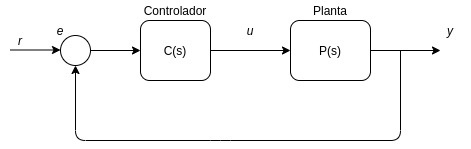
\includegraphics[scale=0.70]{planta.jpg}
	\caption{Planta PID simples}
\end{figure}

De forma resumida, o controlador PID, trabalhando numa malha fechada, tem a estrutura mostrada na imagem acima. A variável $e$ representa o erro, que é a diferença entre a saída desejada $r$ e a saída real $y$. Esse sinal de erro é alimentado para o controlador PID, que calcula tanto a derivada como a integral desse sinal de erro em relação ao tempo. O sinal do controlador, $u$, para a planta é igual ao ganho proporcional $K_p$ vezes a magnitude do erro mais a integral do ganho $K_i$ vezes a integral do erro mais a derivada do ganho $K_d$ vezes a derivada do erro.

\begin{equation}
u(t) = K_pe(t) + K_i\int e(t)\,dt + K_p\frac{de}{dt}
\end{equation}

Esse sinal de controle, $u$, é passado para a planta e a nova saída $y$ é obtida. Essa nova saída é enviada de volta e comparada à referência para que se encontre o novo sinal de erro. O controlador recebe esse novo sinal e atualizada a entrada do controlador. Esse processo continua enquanto o controlador estiver funcionando.

\section{Filtros}

Os filtros têm por objetivo tornar o controle implementado, diminuindo o sobressinal e o tempo para se alcançar o \textit{setpoint}.

\subsection{Filtro derivativo}

O filtro derivativo age no regime transitório. Esse tipo específico de filtro tenta prever alguns comportamentos, eliminando ruídos de alta frequência e suavizando o efeito do ruído no controle. No caso real a queda da água, por exemplo, poderia ser considerada como um ruído, porque essa queda causaria um distúrbio no tanque. Na simulação é um pouco mais difícil de notar esse tipo de comportamento, então, adiantando a parte prática, encontramos um pouco de dificuldade de ver o efeito dele no sistema.

\subsection{Filtro \textit{anti windup}}

Sistemas de controle podem sofrer com resposta transitória lenta e oscilatória se houver, como entrada, um sinal saturado, pois a malha de realimentação é desfeita quando esse valor não é considerado. Isso faz com que a saída demore muito para atingir o \textit{setpoint} e apresente oscilações frequentes, esses dois comportamentos são indesejáveis numa planta industrial. Então, para atacar esse problema existe o filtro \textit{anti windup}, que faz com que o controlador saia da região da saturação e volte para o comportamento esperado.

\section{Sistemas de segunda ordem}

Até aqui foram discutidos os conceitos necessários para a realização da primeira parte do experimento, para a segunda parte serão necessários alguns novos conceitos relacionados aos sistemas de segunda ordem. 

Os sistemas de segunda ordem são aqueles cujo modelo pode ser escrito por uma equação diferencial de segunda ordem, ou seja, os que possuem dois polos \cite{dan_madeira}.

O comportamento dos sistemas de segunda ordem é bastante sensível à mudança nos parâmetros, então é importante fazer uma classificação dos perfis existentes para esses sistemas, tentando entender melhor os fenômenos que ocorrem em cada caso. Durante as simulações foi notado que apesar de haver bastante matemática por trás dos modelos, muita coisa pode ser entendida de forma mais fácil de forma empírica, alterando os parâmetros e analisando a mudança nos gráficos.

Existem três tipos principais de sistemas de segunda ordem, são eles:
\begin{enumerate}
	\item Superamortecido: um polo na origem, proveniente da entrada degrau unitário e dois polos reais;
	
	\item Subamortecido: um polo na origem proveniente da entrada degrau unitário e dois polos complexos, vindos do sistema;
	
	\item Criticamente amortecido: um polo na origem proveniente da entrada degrau unitário e dois polos reais iguais.		
\end{enumerate}

\subsection{Sistemas de segurança}

No segundo experimento será necessário implementar um sistema de segurança que impeça a água de transbordar, mas a bomba também não pode trabalhar sem água, numa situação real ela poderia queimar. Então será feito um sistema de segurança que não permita nem que haja um transbordamento nem uma quebra do motor. 

Esse tipo de segurança é definido como sendo um conjunto de passos, na lógica de automação e controle, que devem existir para garantir a segurança de um equipamento, pessoa ou processo \cite{meneghetti1}. Nesses casos as travas lógicas, que são implementadas em \textit{software} e as travas físicas, que são \textit{hardware}, são usadas para garantir a segurança das pessoas e a continuidade da produção.

O sistema vai monitorar certas condições da planta, tentando mante-la dentro do limite operacional estabelecido, e quando condições de risco, ou que estiverem fora dos parâmetros criados, forem detectadas ele deve acionar alarmes, ou também pode atuar nos erros.

Na simulação as seguintes regras devem ser seguidas e implementadas no sistema de segurança:

\begin{itemize}
	\item Não deve ser enviado para o sistema uma tensão fora dos limites de $\pm 4V$;
	\item A bomba não pode trabalhar sem que haja líquido a ser bombeado;
	\item Nenhum dos dois tanques pode transbordar.
\end{itemize}

\section{Controle em cascata}

O controle em cascata é implementado quando a malha de controle simples não responde satisfatoriamente, principalmente em processos que possuem uma perturbação contínua em torno da variável que se deseja manipular, ou seja, o nível do tanque 2 com o constante recebimento de água a partir do tanque 1 pode se encaixar nessa situação. O controle em cascata consiste de um controlador primário que regula um controlador secundário, melhorando a velocidade de resposta e reduzindo os distúrbios causados pela malha secundária

No arranjo proposto pelo roteiro pode-se manipular a tensão enviada para a bomba e obter o nível desejado no tanque 1, que influencia na vazão de saída afetando a vazão de entrada do tanque 2. O objetivo é controlar o nível do segundo tanque a partir do primeiro, então com uma malha externa de controle é preciso captar o erro entre a referência desejada e o nível do tanque 2 e fornecer um valor para o tanque 1, alterando a tensão do motor e aumentando, ou diminuindo, o nível do segundo tanque.
\chapter{Desenvolvimento e resultados}

O experimento consiste dos seguintes pontos:
\begin{enumerate}
    \item Implementar a ação proporcional, formando controladores P, e realizar testes com diferentes valores de ganho;
    \item Realizando testes em cada etapa, faça o proposto:
    \begin{enumerate}
        \item Implemente a ação integrativa, formando controladores PI;
        \item Implemente a ação derivativa, permitindo agora formar controladores PD e PID;
        \item Implemente o filtro na ação derivativa;
        \item Implemente o filtro \textit{anti-reset-windup}.
    \end{enumerate}
    \item Descrever a diferença no comportamento do sistema com cada uma das leis de controle implementada. Levando em consideração as entradas degrau e senoide;
    \item Para cada lei de controle, verificar e descrever o comportamento do sistema para diferentes valores dos ganhos.
\end{enumerate}
% ---
\section{Implementação da ação proporcional - controlador P}

Como foi dito anteriormente, esse é o controlador mais simples, pois o sinal de saída é proporcional ao erro. Para implementar esse tipo de controlador basta colocar um ganho entre o comparador e o bloco de saturação.

\begin{figure}[h]
	\centering
	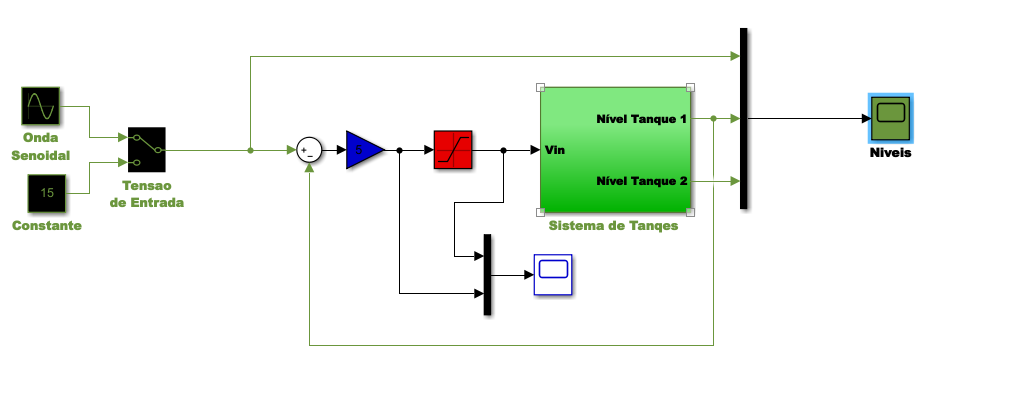
\includegraphics[scale=0.70]{controlador_p.PNG}
	\caption{Controlador Proporcional}
\end{figure}
\newpage

Com isso feito, a simulação apresenta o seguinte comportamento de acordo com os ganhos.

\subsection{Controlador P - ganho 1}

O controlador P é o mais simples, ele apenas vai tentar compensar o erro de forma proporcional. Começamos com ganho unitário, ou seja, praticamente não haverá correção do erro.

\begin{figure}[h]
	\centering
	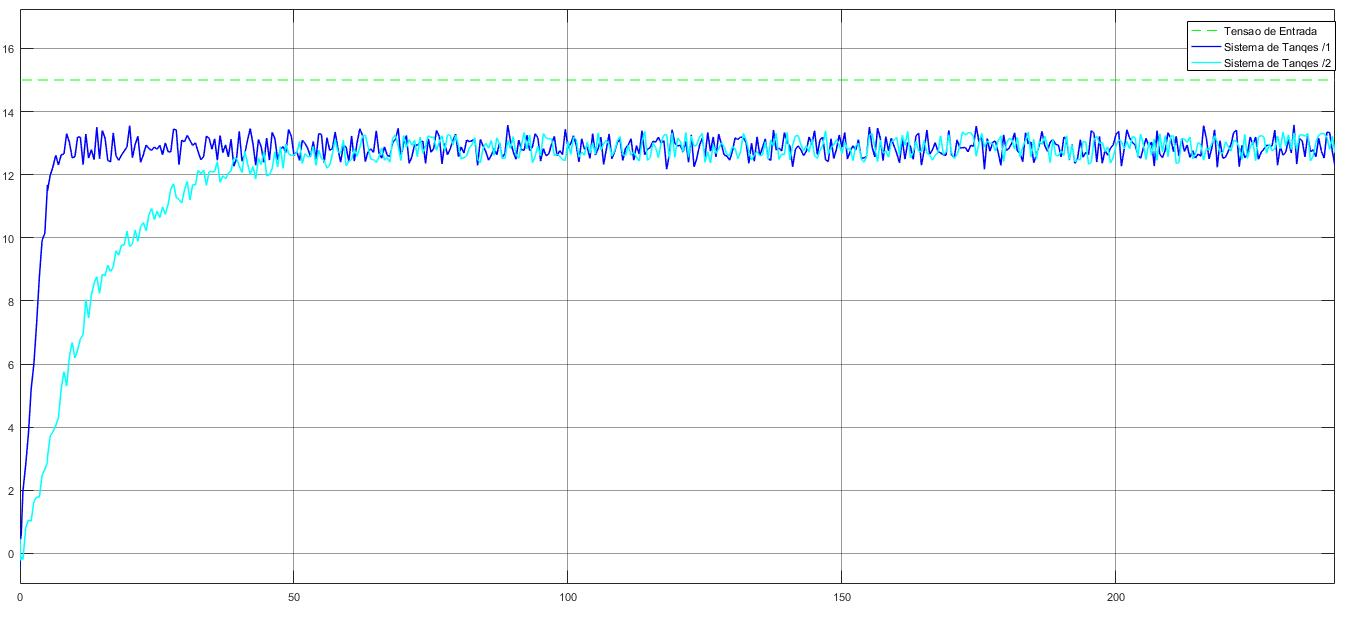
\includegraphics[scale=0.30]{controlador_p_ganho_1.jpg}
	\caption{Controlador P - Ganho 1}
\end{figure}

Na imagem acima é possível ver que o ganho unitário não alcança o valor desejado, então fica abaixo do que seria ideal, 15. Não há muito o que discutir nesse caso, mas nos próximos ganhos, de 5 e 10, veremos diferenças.

\begin{figure}[h]
	\centering
	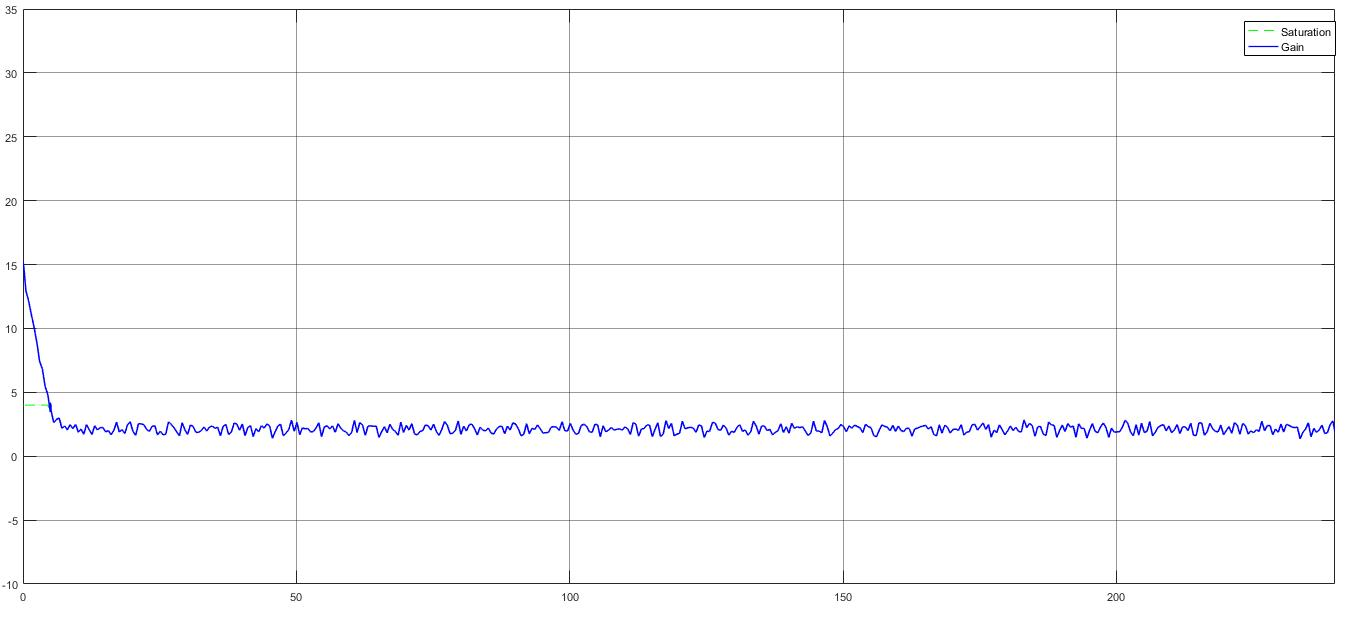
\includegraphics[scale=0.30]{osciloscopio_ganho_1.jpg}
	\caption{Controlador P Ganho 1 - Sinal de entrada}
\end{figure}

\subsection{Controlador P - ganhos 5 e 10}

No caso de ganhos maiores, 5 e 10 no exemplo apresentado, o controlador vai aplicar esses valores tentando corrigir o erro encontrado, se o ganho for muito alto, o controlador vai aplicar "mais vezes" tentando compensar a maior distância em relação ao valor ideal, de novo, 15. Esse comportamento pode ser visto no nível, como mostrado a seguir.

\begin{figure}[h]
	\centering
	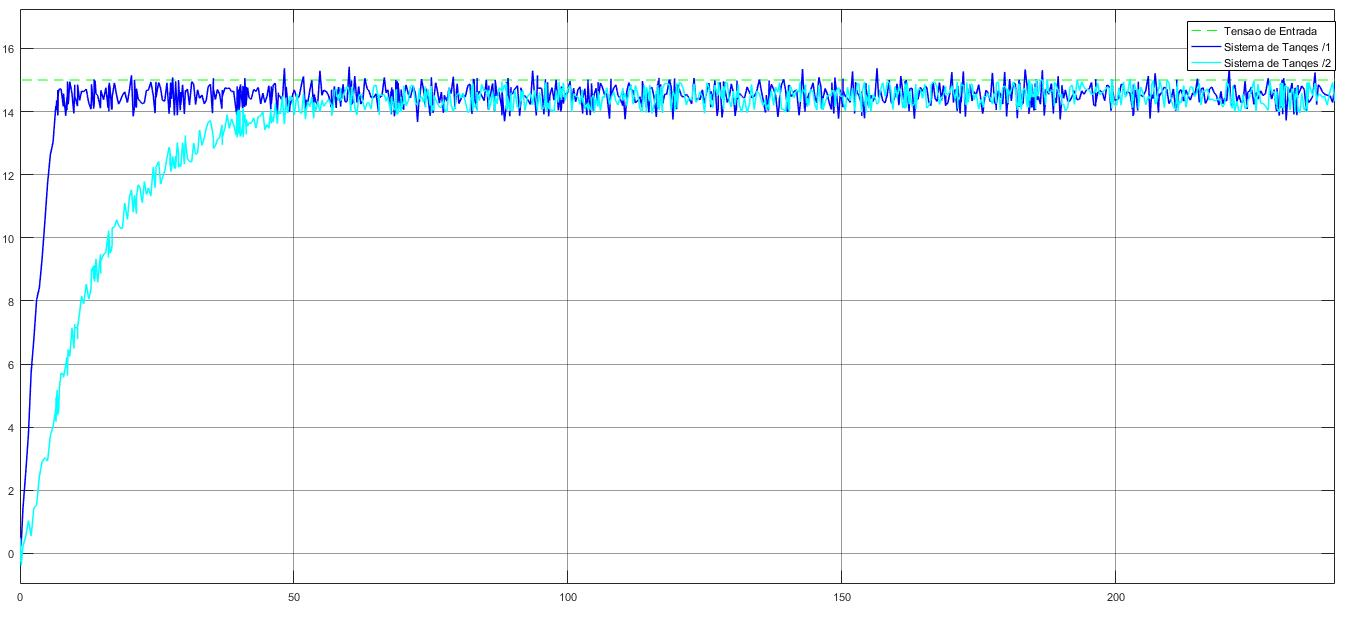
\includegraphics[scale=0.30]{controlador_p_ganho_5.jpg}
	\caption{Controlador P - Ganho 5}
\end{figure}

\begin{figure}[h]
	\centering
	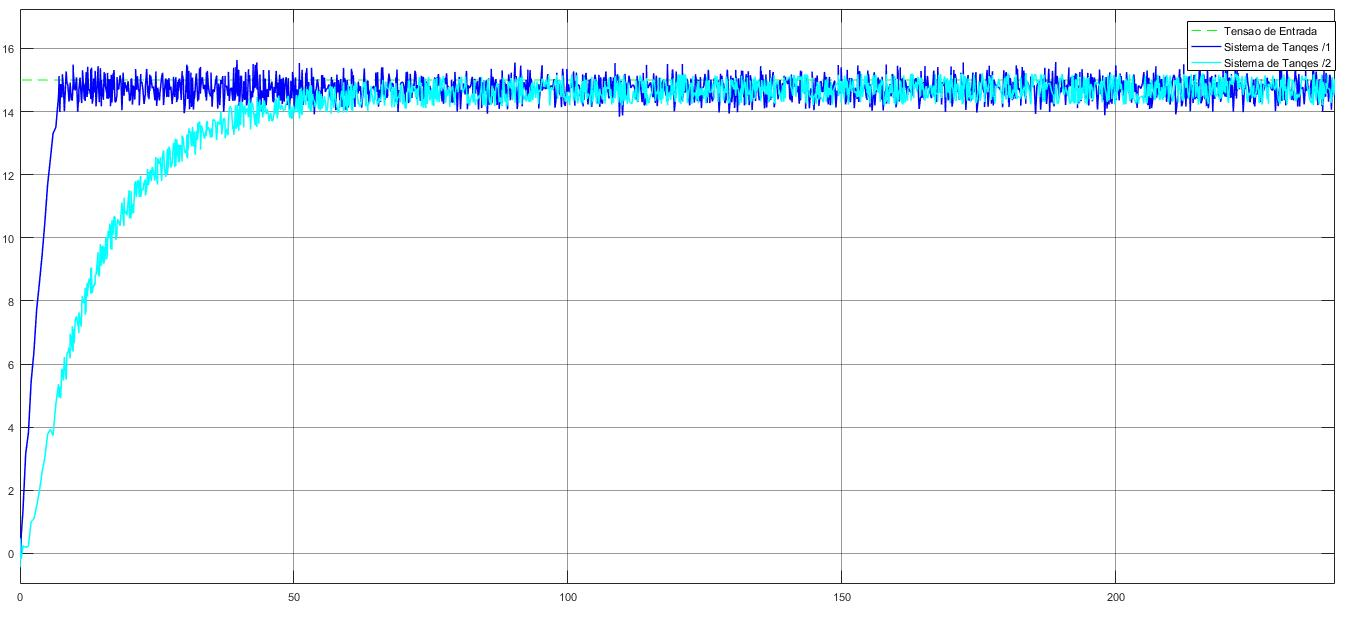
\includegraphics[scale=0.30]{controlador_p_ganho_10.jpg}
	\caption{Controlador P - Ganho 10}
\end{figure}

E também pode ser visto no sinal do controlador, como pode ser visto abaixo.

\begin{figure}[h]
	\centering
	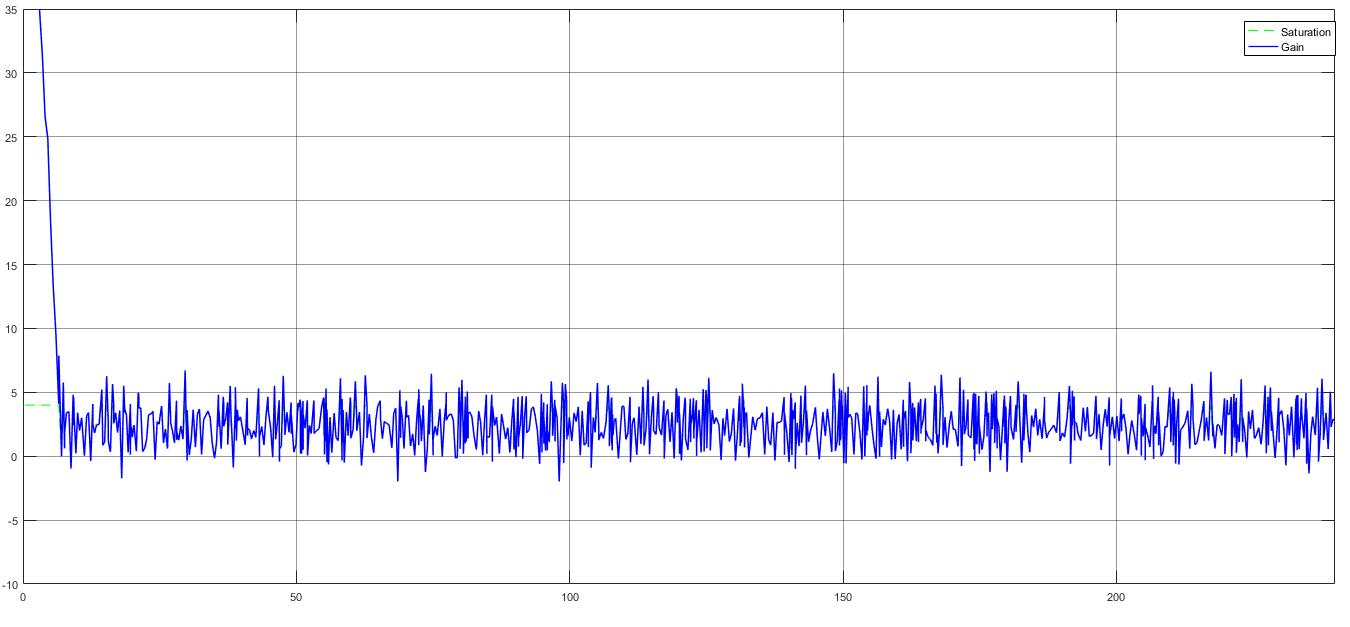
\includegraphics[scale=0.33]{osciloscopio_ganho_5.jpg}
	\caption{Controlador P Ganho 5 - Sinal de entrada}
	\label{fig:controladorPG5}
\end{figure}

\begin{figure}[h]
	\centering
	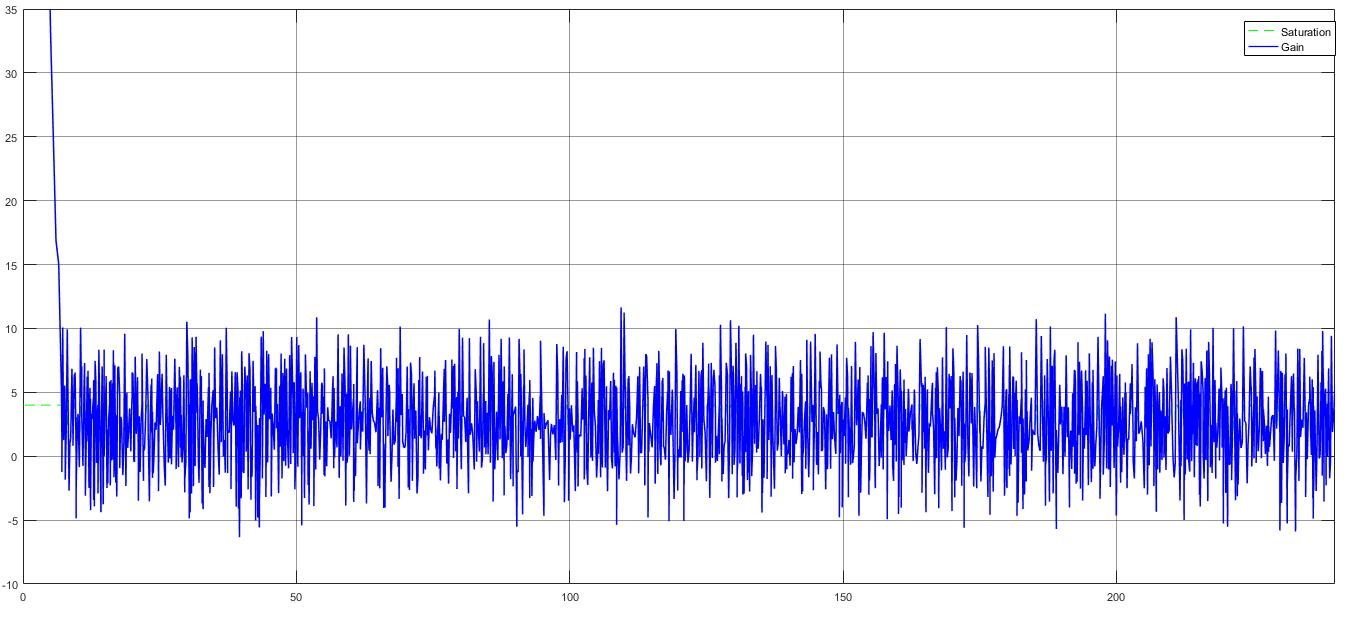
\includegraphics[scale=0.33]{osciloscopio_ganho_10.jpg}
	\caption{Controlador P Ganho 10 - Sinal de entrada}
	\label{fig:controladorPG10}
\end{figure}

O comportamento de compensação do ganho fica muito nítido quando comparamos as figuras \ref{fig:controladorPG5} e \ref{fig:controladorPG10}, em que o Controlador com Ganho 10 aplica o sinal de forma mais frequente e tem uma amplitude maior também, justamente porque o ganho é muito alto e a cada vez que ele aplica esse ganho se distancia bastante do valor que precisa atingir, então aplica um sinal novamente e, de novo, se distancia do objetivo. Esse comportamento se repete constantemente e gera as imagens que podemos analisar.

\clearpage
\section{Expansão do controlador}

Nessa parte, ainda nos sistemas de primeira ordem, vamos expandir o controlador, adicionando os componentes Integrador e Derivativo. Para realizar esses experimentos, construímos uma simulação já com os três componentes do controlador PID, e quando queríamos apenas um PD, por exemplo, deixamos o $K_i$ igual a 0, então não havia influência do Integrador no sistema. 

A simulação usada foi construída usando como base o arquivo disponibilizado no SIGAA.

\begin{figure}[h]
	\centering
	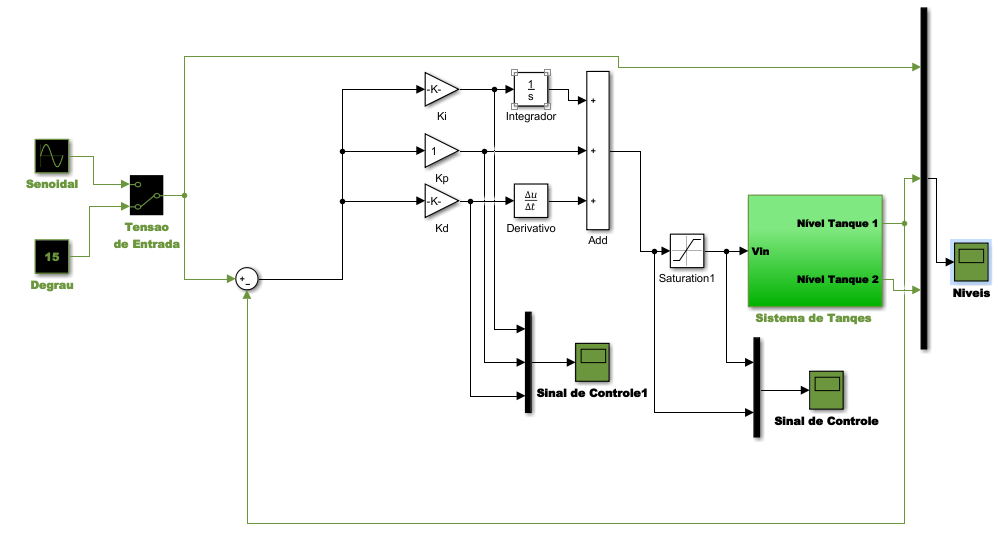
\includegraphics[scale=0.55]{Controlador_pid.PNG}
	\caption{Controlador PID no Simulink}
	\label{fig:controladorPID}
\end{figure}

\subsection{Implementação da ação integrativa - controlador PI}

O termo integral é proporcional à magnitude do erro e à duração do erro. De forma mais detalhada, a integral no PID é a soma dos erros ao longo do tempo, esse termo vai tentar corrigir os erros deslocando a curva. Ele vai acelerar a aproximação ao \textit{setpoint}, e por isso pode causar um \textit{overshoot}. Usamos os valores da tabela \ref{tab:tabelaPI} no experimento.

\begin{table}[h]
\centering
\begin{tabular}{ccc}
\multicolumn{0}{c}{} $K_p$ & $K_i$ & $K_d$ \\\hline
                    1,0 & 0,01 & 0 \\
                    1,0 & 0,02 & 0 \\
                    2,0 & 0,01 & 0
\end{tabular}
\caption{Valores do controlador PI}
\label{tab:tabelaPI}
\end{table}

\begin{figure}[h]
	\centering
	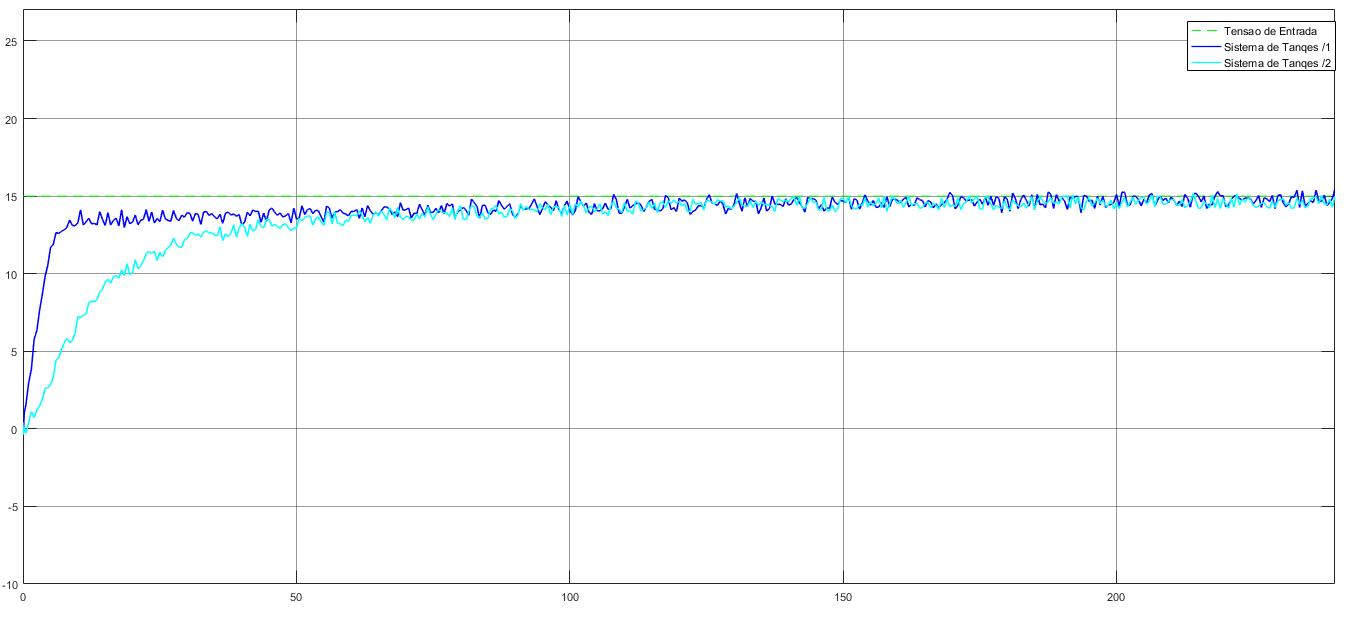
\includegraphics[scale=0.30]{1 - nivel_PI_1kp_001ki.jpg}
	\caption{Controlador PI - nível dos tanques - $K_p = 1$ e $K_i = 0,01$}
	\label{fig:controladorPI_1}
\end{figure}

\begin{figure}[h]
	\centering
	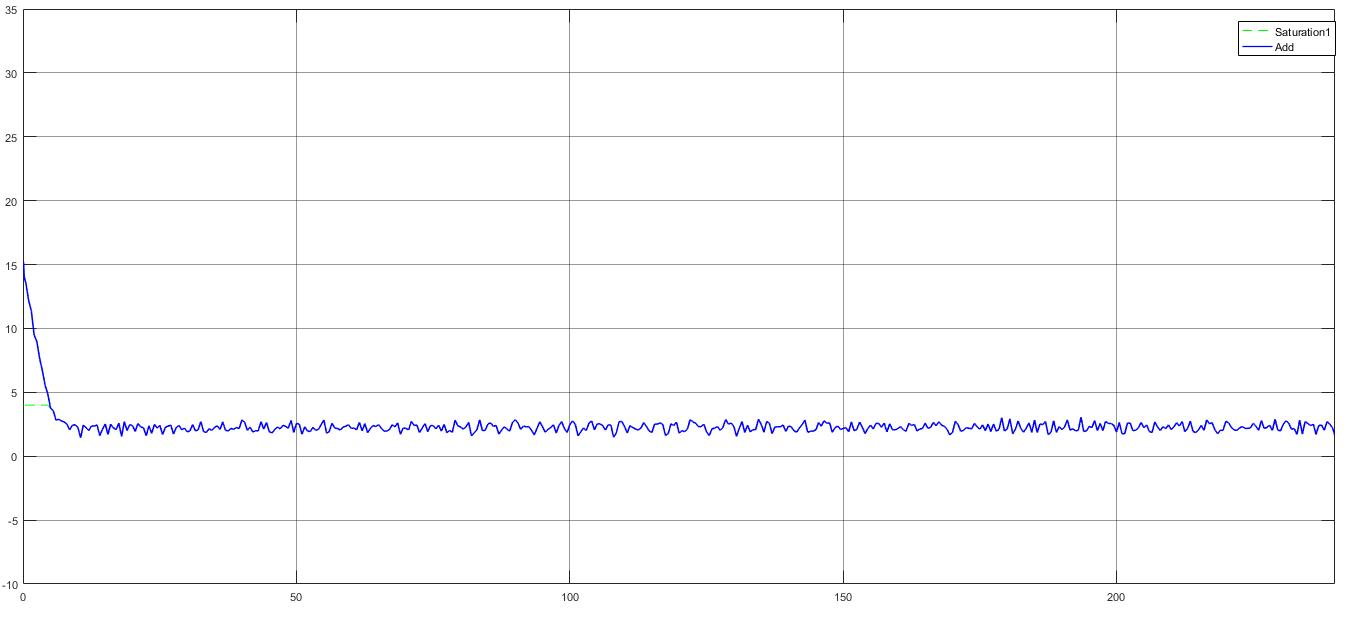
\includegraphics[scale=0.30]{1 - PI sinal_controle.jpg}
	\caption{Controlador PI - sinal de controle - $K_p = 1$ e $K_i = 0,01$}
	\label{fig:sinal_controladorPI_1}
\end{figure}

\begin{figure}[h]
	\centering
	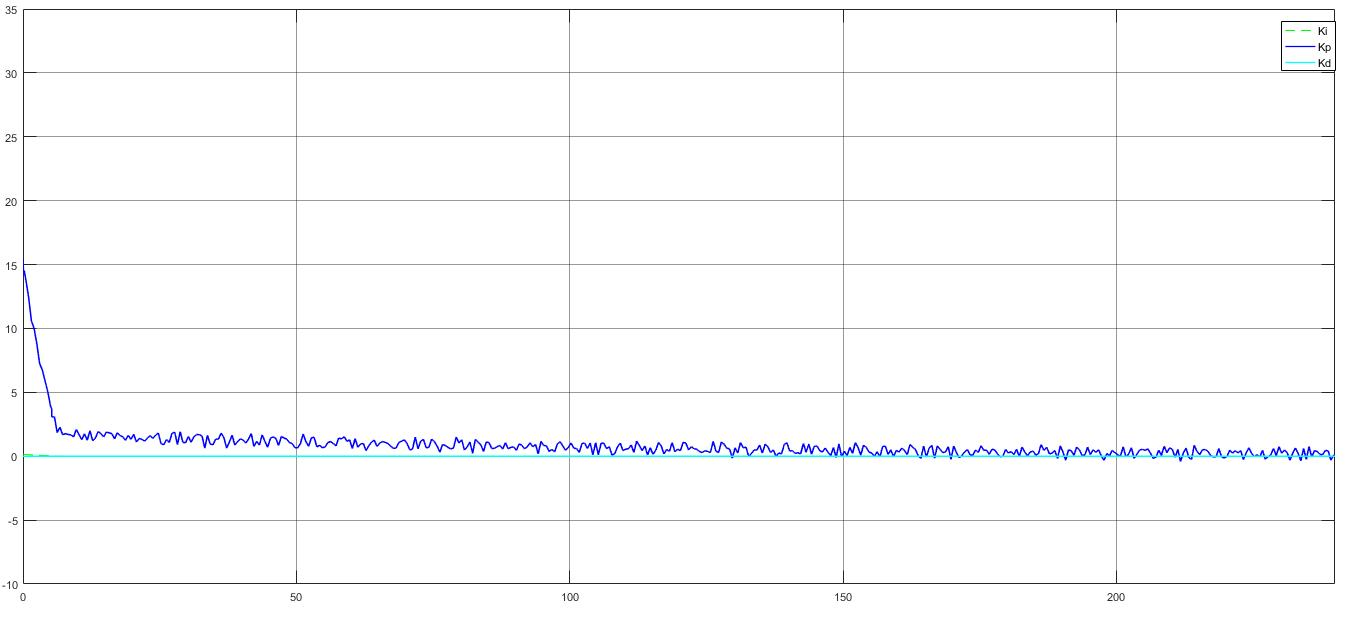
\includegraphics[scale=0.30]{1 - PI acoes_controle.jpg}
	\caption{Controlador PI - ações de controle - $K_p = 1$ e $K_i = 0,01$}
	\label{fig:acao_controladorPI_1}
\end{figure}


\clearpage

Nas imagens \ref{fig:controladorPI_1}, \ref{fig:sinal_controladorPI_1} e \ref{fig:acao_controladorPI_1} é possível notar que o controlador demorou um pouco mais que o tipo P somente para alcançar o \textit{setpoint}, mas uma vez alcançado, o comportamento é bem definido e estável, no sentido de não se distanciar mais do objetivo. É importante testar um controlador com o $K_p$ alto para ver o impacto que o $K_i$ pode causar.

\subsection{Implementação da ação derivativa - controlador PD e PID}

A ação derivativa tenta prever o comportamento do sistema diminuindo o tempo em que se alcança a estabilidade. E esse foi o comportamento notado quando aplicamos a ação derivativa, uma diminuição de aproximadamente 50\% para se alcançar a estabilidade, e uma diminuição do \textit{overshoot}, em alguns casos o \textit{overshoot} nem acontecia.

\begin{figure}[h]
	\centering
	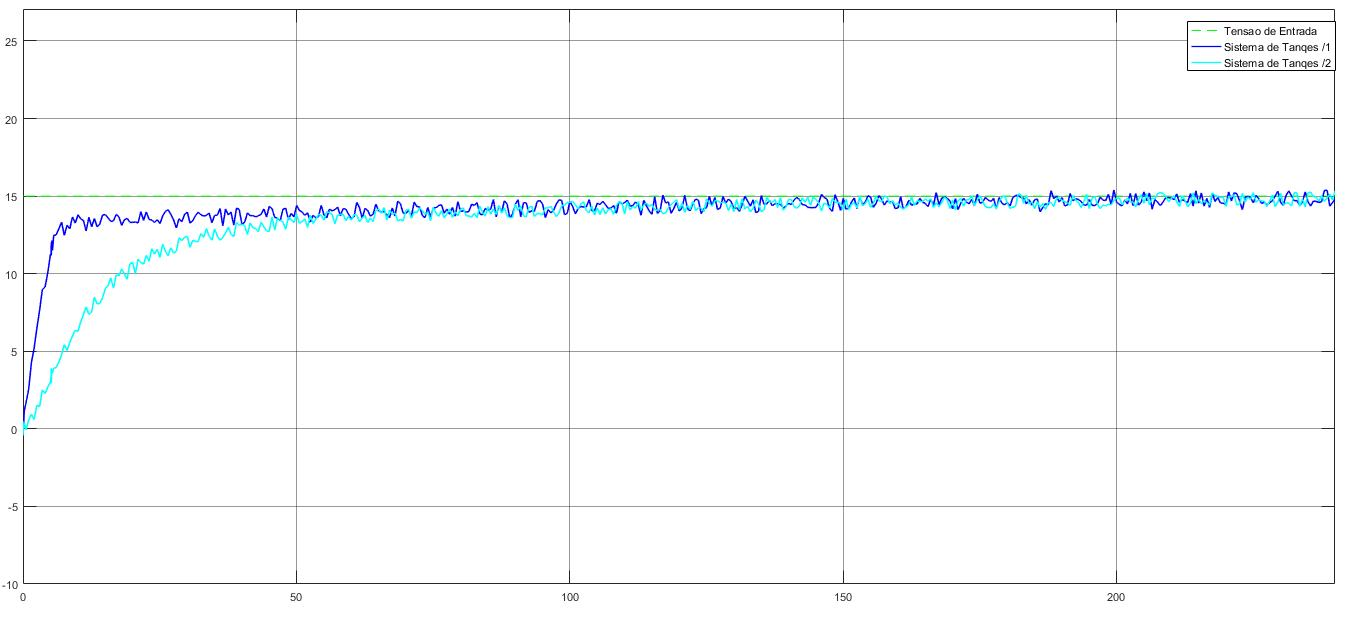
\includegraphics[scale=0.30]{4 - nivel_ PDI_1kp_001ki_0001kd.jpg}
	\caption{Controlador PID - nível dos tanques - $K_p = 1$, $K_i = 0,01$ e $K_d=0,001$}
	\label{fig:controladorPID_1}
\end{figure}

\begin{figure}[h]
	\centering
	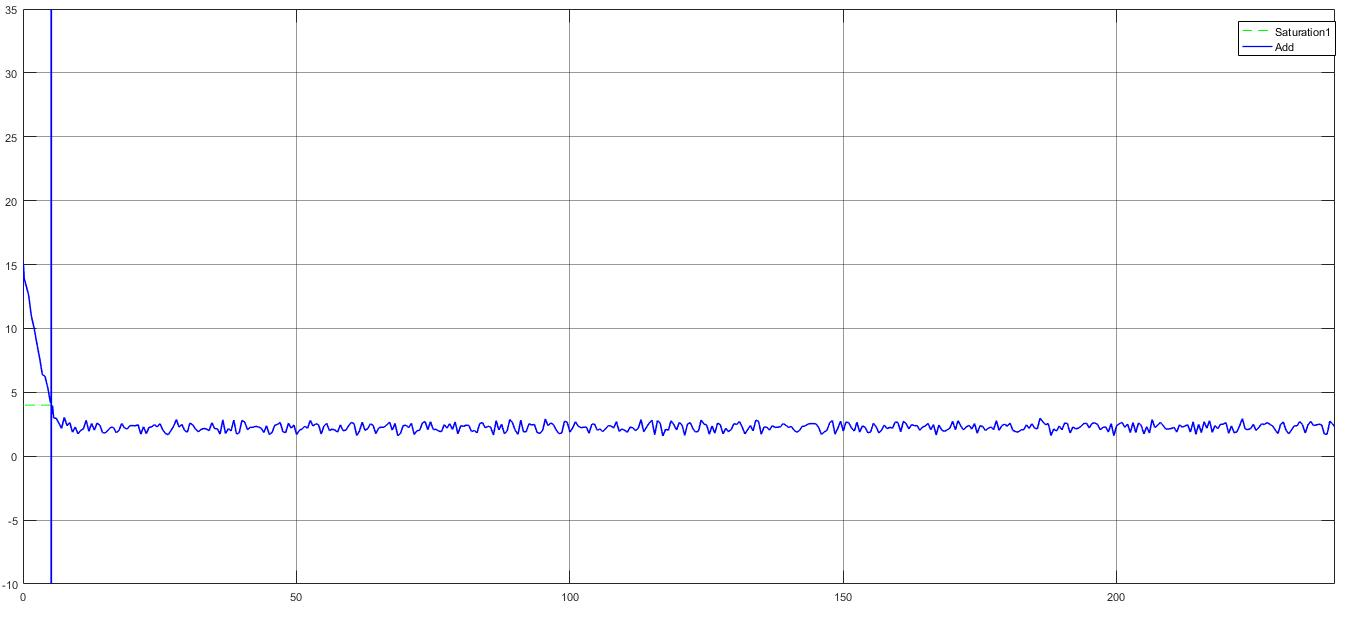
\includegraphics[scale=0.30]{4 - PDI sinal_controle.jpg}
	\caption{Controlador PI - sinal de controle - $K_p = 1$, $K_i = 0,01$ e $K_d=0,001$}
	\label{fig:sinal_controladorPID_1}
\end{figure}

\begin{figure}[h]
	\centering
	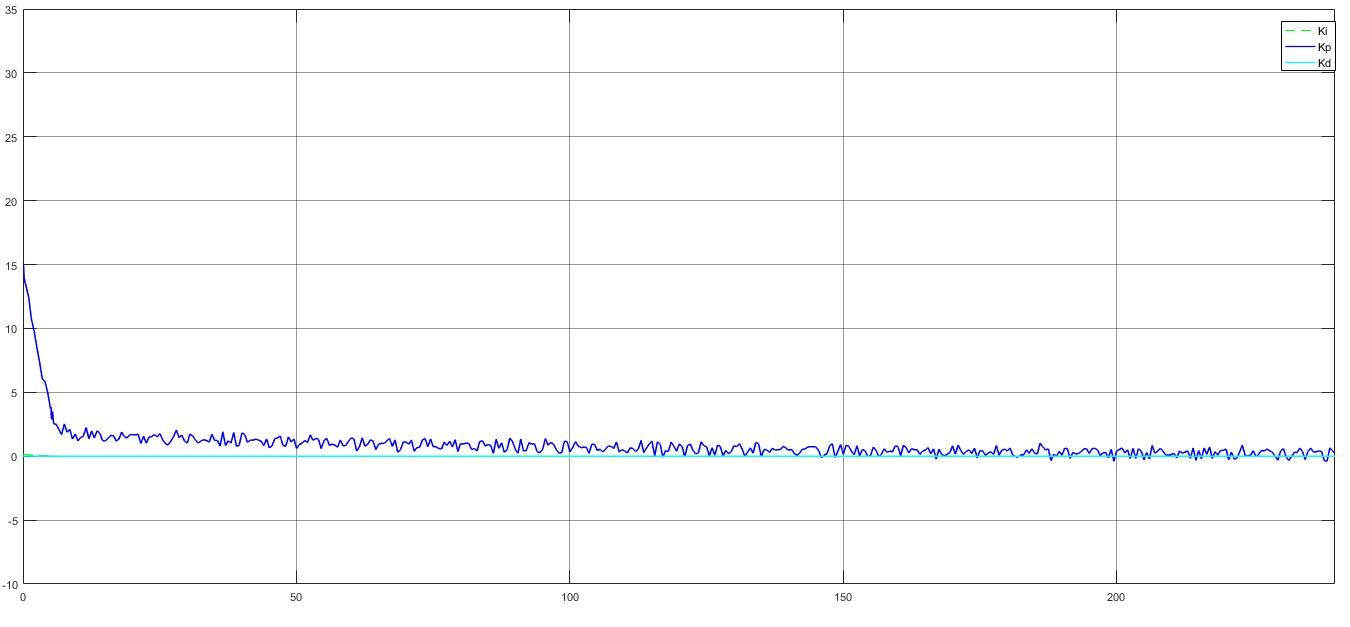
\includegraphics[scale=0.30]{4 - PDI acoes_controle.jpg}
	\caption{Controlador PI - ações de controle - $K_p = 1$, $K_i = 0,01$ e $K_d=0,001$}
	\label{fig:acao_controladorPID_1}
\end{figure}

\begin{figure}[h]
	\centering
	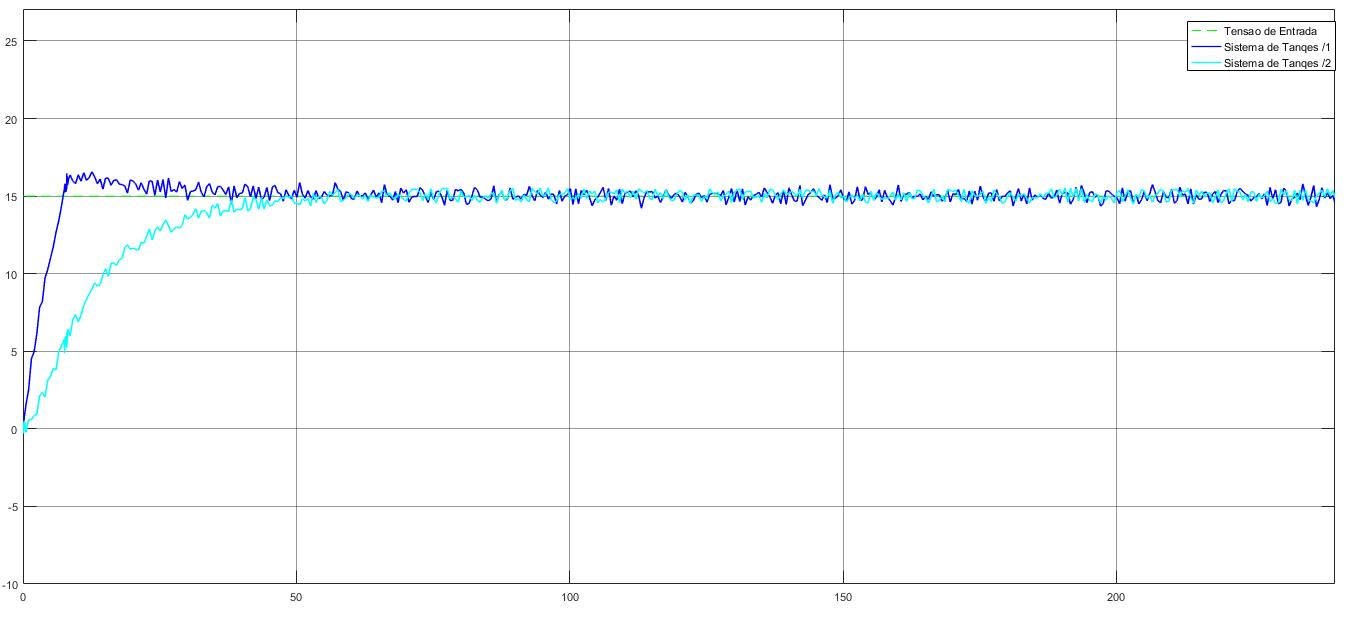
\includegraphics[scale=0.30]{6 - nivel_ PDI_2kp_01ki_0001kd.jpg}
	\caption{Controlador PID - nível dos tanques - $K_p = 2$, $K_i = 0,01$ e $K_d=0,001$}
	\label{fig:controladorPID_2}
\end{figure}

O \textit{overshoot} pode ser visto na figura \ref{fig:controladorPID_2}. Então o conjunto das três ações possíveis trabalha bem, diminuindo o \textit{overshoot} e diminuindo o tempo para se alcançar a estabilidade.

\clearpage
\subsection{Implementação do filtro na ação derivativa}

No filtro de ação derivativa obtivemos resultados que não foram muito satisfatórios, mesmo alterando os valores dos coeficientes o comportamento era praticamente o mesmo. Apesar de ter apresentado um menor tempo para alcançar a acomodação, a diferença não foi grande, o melhor ponto que pode ser citado aqui é a diminuição do sobressinal.

\begin{figure}[h]
	\centering
	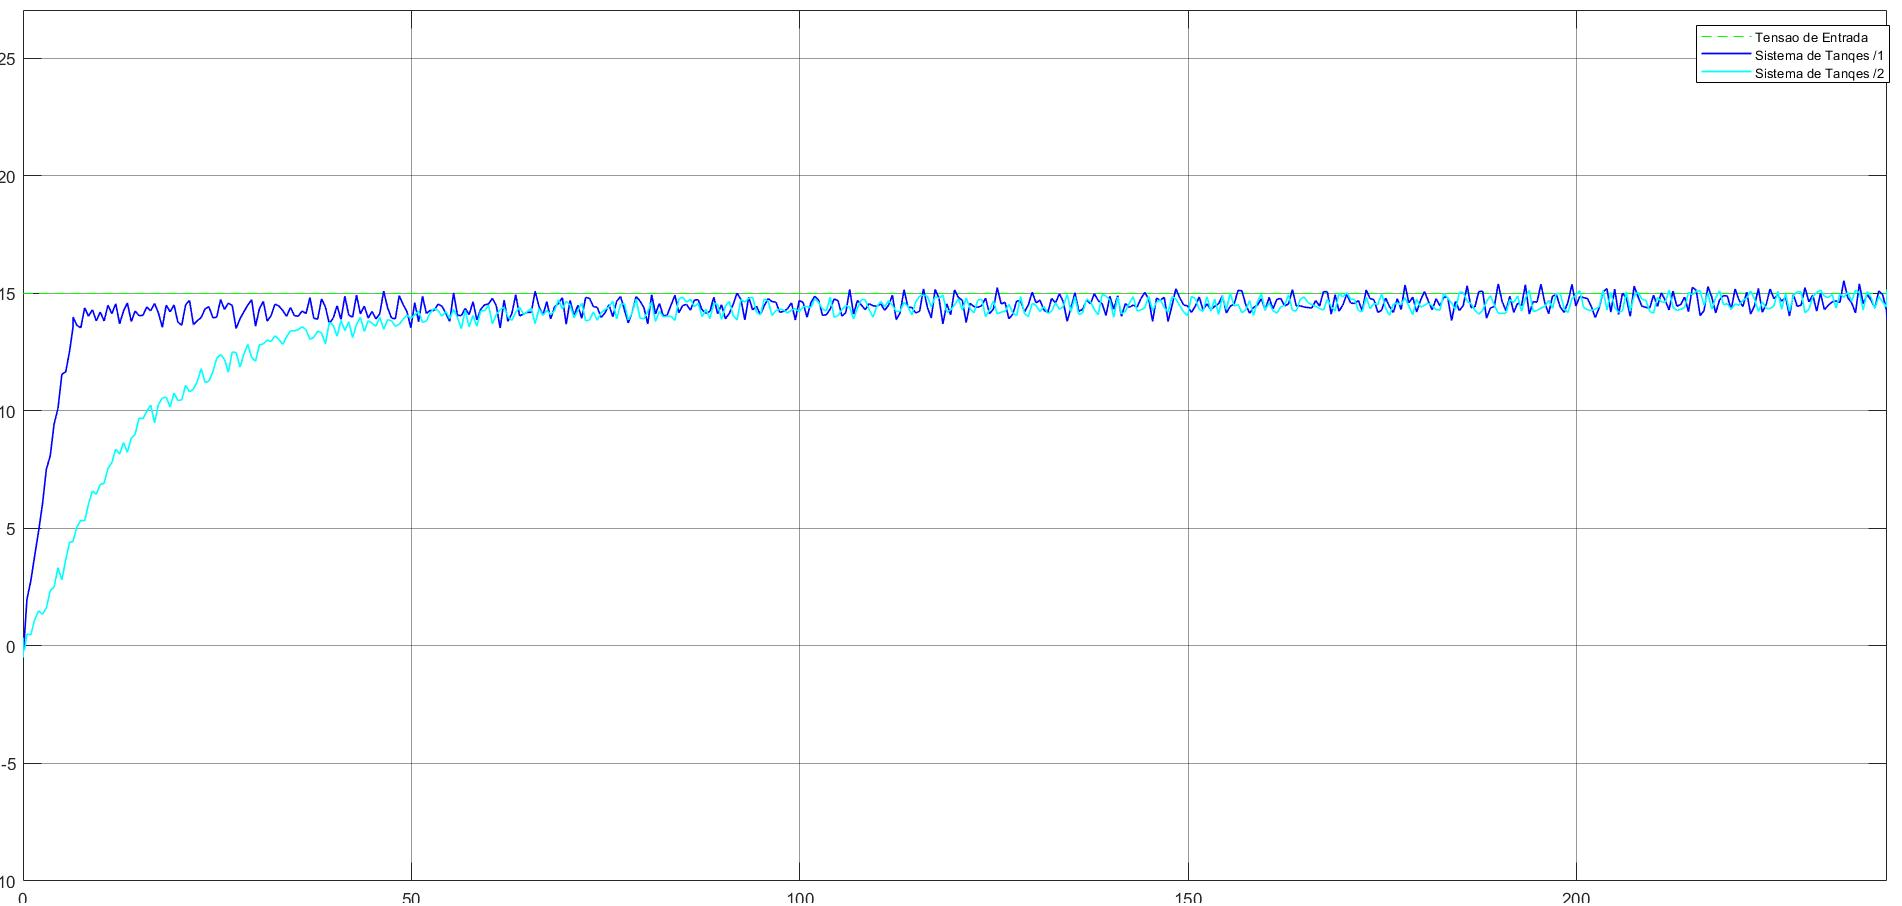
\includegraphics[scale=0.20]{Filtro_derivativo_1.jpg}
	\caption{Filtro derivativo}
\end{figure}

\subsection{Implementação do filtro \textit{anti-reset-windup}}

O filtro \textit{anti windup} deveria apresentar um sinal melhor que o controlador PID simples, em resumo, ele deveria apresentar menor sobressinal e menor tempo para atingir a estabilidade, porém, obtivemos um comportamento semelhante ao filtro de ação derivativa. Apesar de realmente apresentar uma melhora, é uma mudança muito pequena em relação ao controlador PID convencional, talvez numa planta industrial real a dificuldade de se implementar um filtro desses e o aumento na complexidade da manutenção não compensem o ganho marginal do sinal.

\begin{figure}[h]
	\centering
	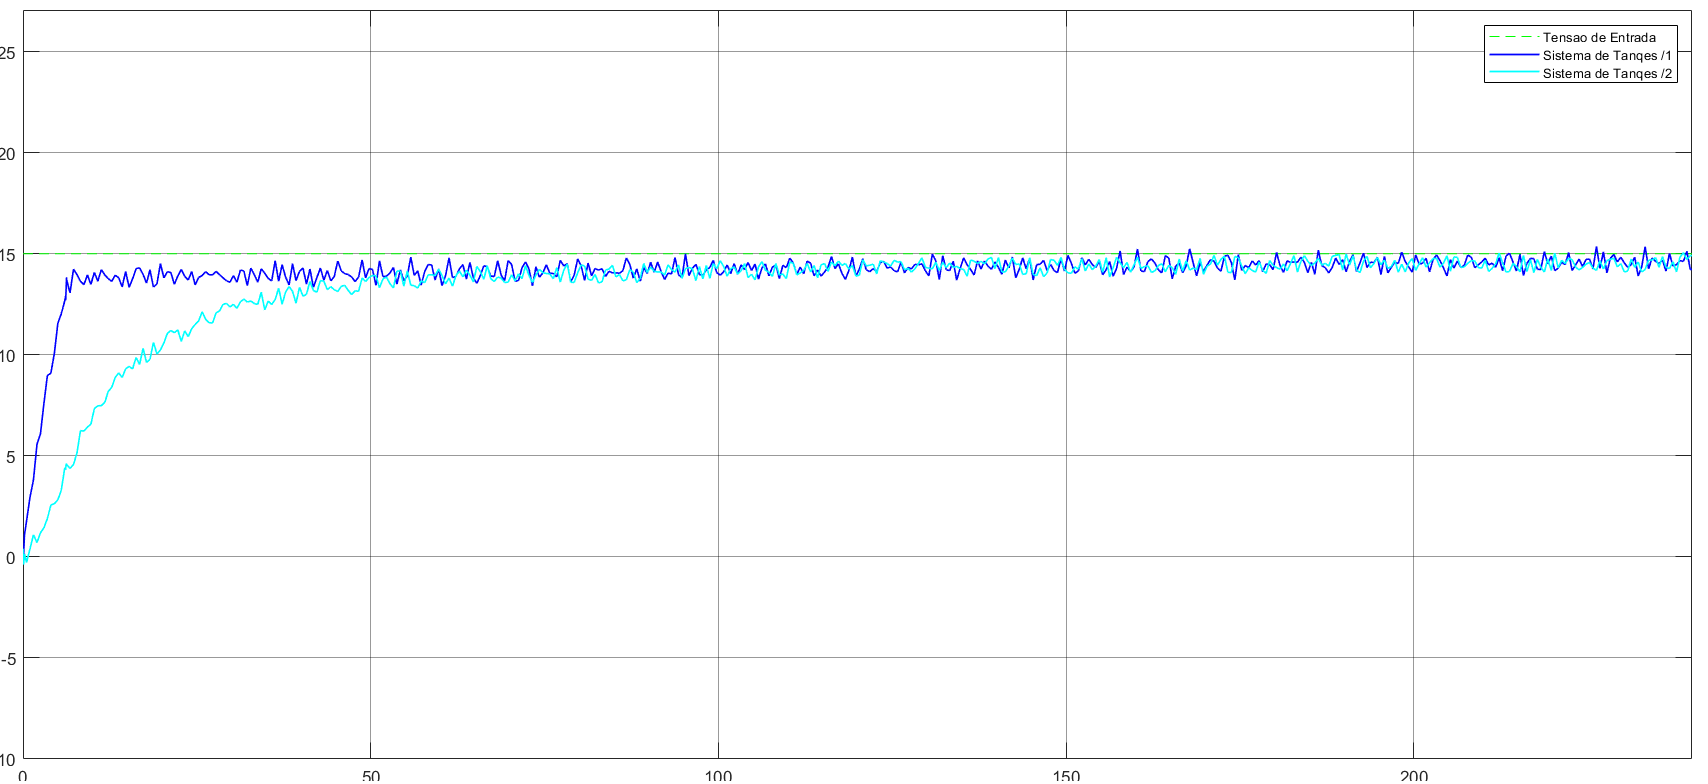
\includegraphics[scale=0.25]{Filtro_windup_1.png}
	\caption{Filtro \textit{anti windup}}
\end{figure}

\section{Controlador de Segunda Ordem}
 
\subsection{Implementação do controlador proporcional em segunda ordem}
 
Os testes começaram com a implementação do controlador proporcional, testamos com o $K_p = 1,0$, e obtemos os seguintes resultados:

\begin{figure}[h]
	\centering
	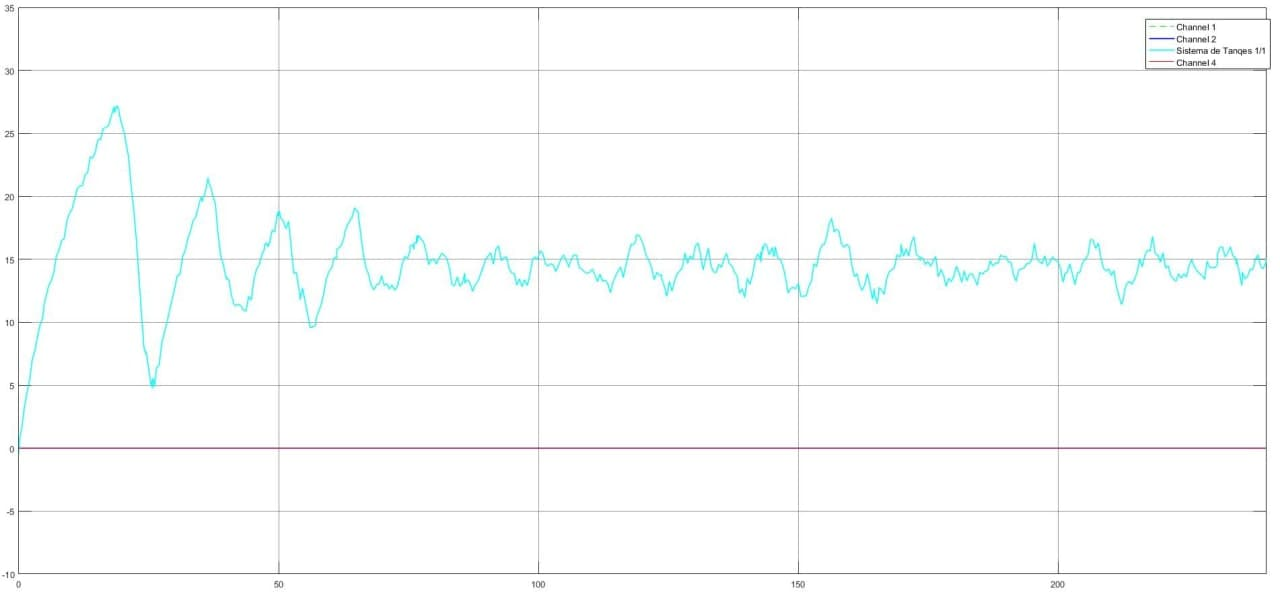
\includegraphics[scale=0.50]{7 - controlador_P_SO.jpg}
	\caption{Controlador P - Sistema de Segunda Ordem}
\end{figure}

\begin{figure}[h]
	\centering
	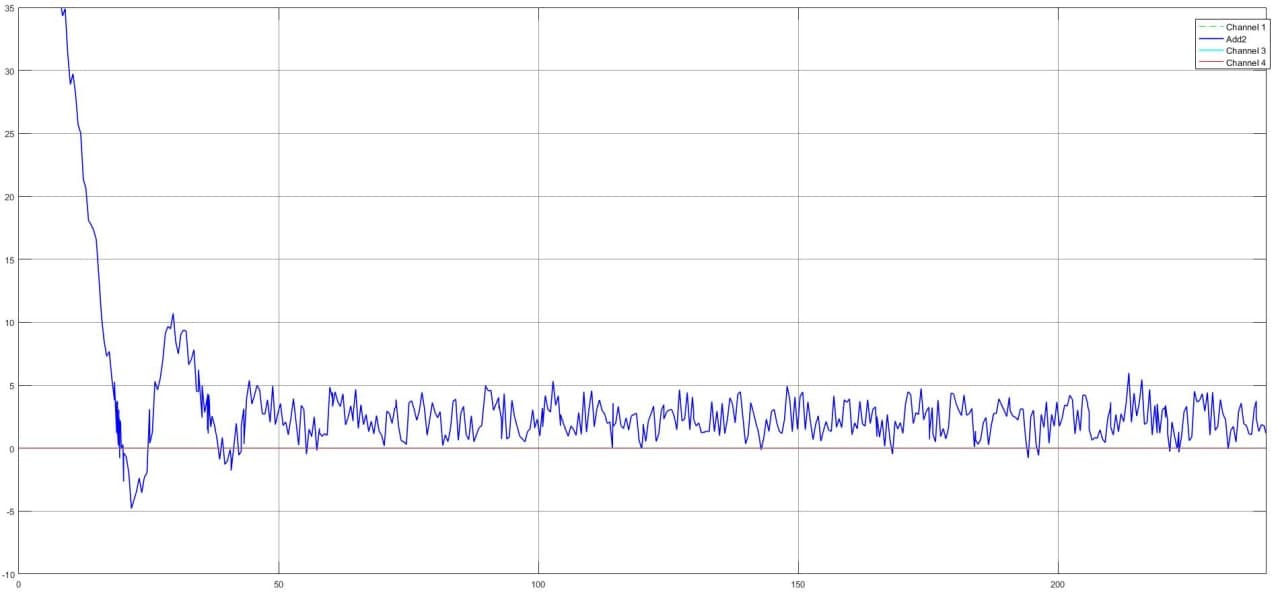
\includegraphics[scale=0.50]{7 - sinal_controle_P_SO.jpg}
	\caption{Sinal de controle - Sistema de Segunda Ordem}
\end{figure}

O comportamento, no geral, é o esperado para essa situação porque o aumento do $K_p$ torna o sistema bastante oscilatório e o erro de regime fica menor. O sinal de entrada começa em 35V e fica saturando por aproximadamente 25s, depois se torna bastante oscilatório. Após isso usamos um $K_p=5,8$. O sistema teve um \textit{overshoot} alto, porém houve menos oscilação e o erro de regime aumentou. 

Como foi mostrado, não é recomendado controlar um sistema por meio de um controlador proporcional simples, porque com o aumento do $K_p$ o erro de regime é reduzido ao custo de um sistema com mais oscilação. Comparando isso com uma possível aplicação do mundo real teríamos um sistema que não consegue manter uma boa reprodutibilidade de peças, por exemplo, elas estariam sempre próximo ao desejado, mas apresentariam diferenças entre si. 

\subsection{Implementação do controlador proporcional integral em segunda ordem}

O controlador PI, como já foi dito, é a soma da ação proporcional com a integral, então com essa união a resposta transitória e o erro de regime melhoram, isso é causado pela ação proporcional e integral, respectivamente. Os testes usaram valores de $K_p=3,0$ e $K_i=0,015$.

\begin{figure}[h]
	\centering
	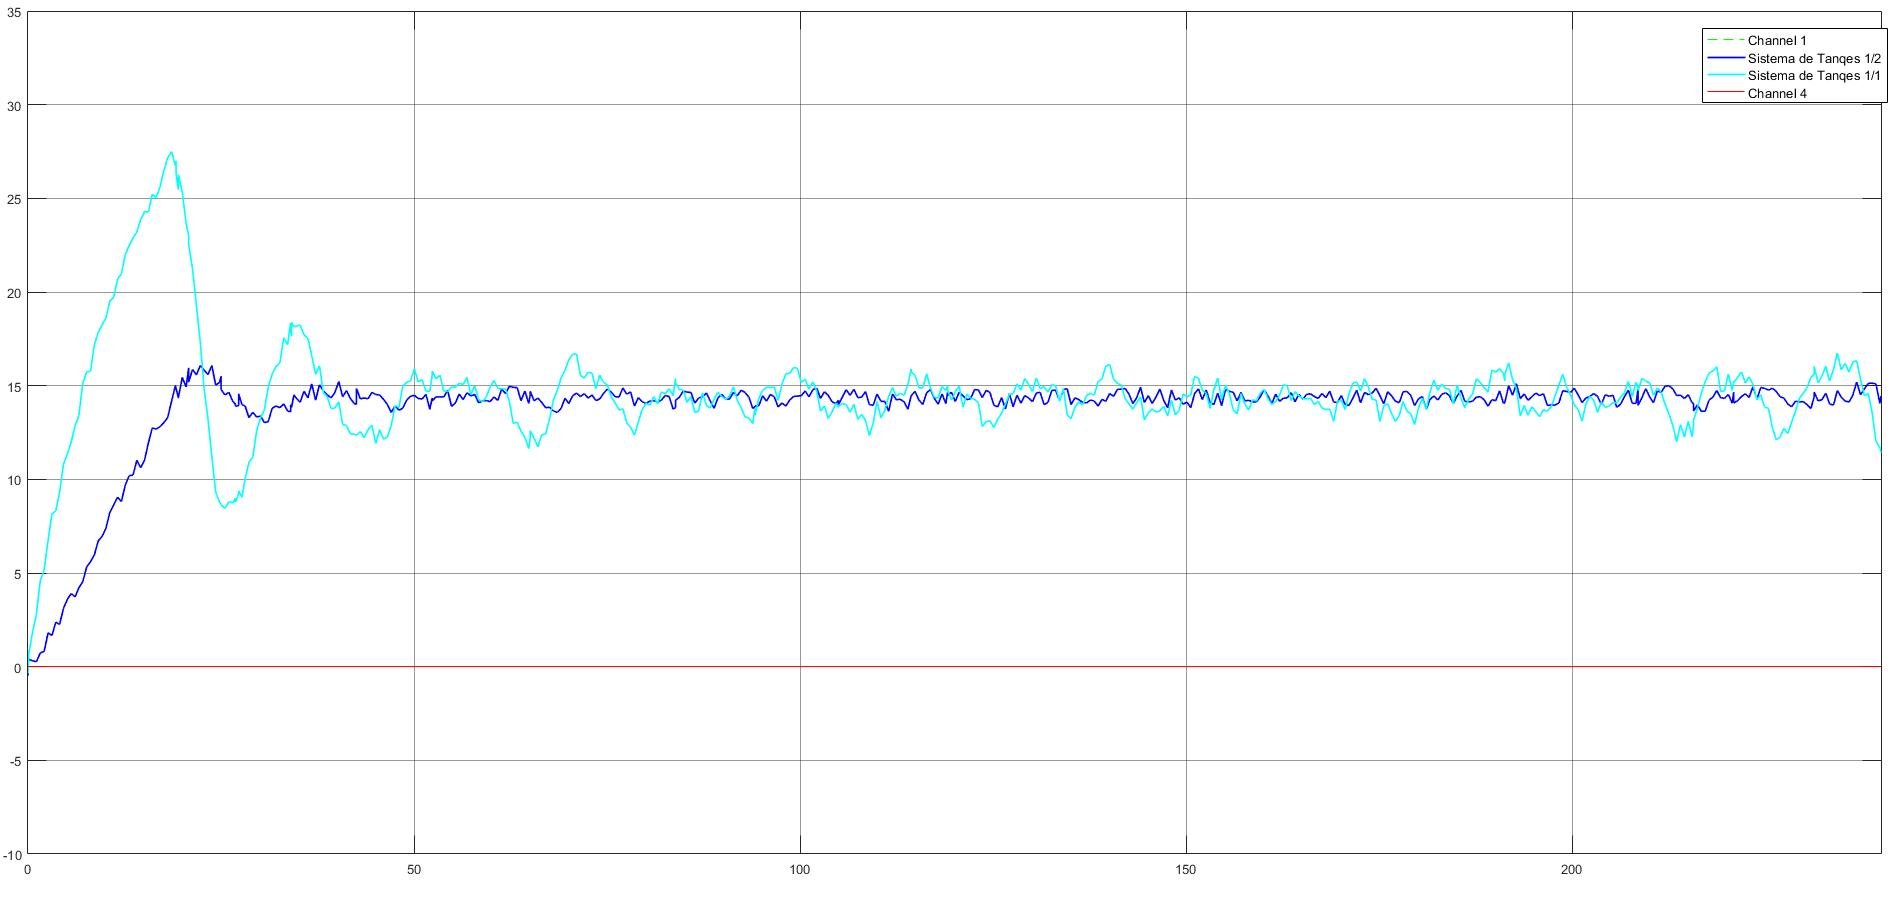
\includegraphics[scale=0.25]{9 - pi_1_segunda_ordem.jpg}
	\caption{Controlador PI - Sistema de Segunda Ordem}
\end{figure}

Os valores resultaram num \textit{overshoot} alto, no tanque 1, mas no tanque 2 foi baixo. Notamos que o sinal oscila bastante, mas esse comportamento tem se repetido ao longo dos experimentos. Apesar desses problemas, o sistema alcança a estabilidade antes dos 25 segundos.

\begin{figure}[h]
	\centering
	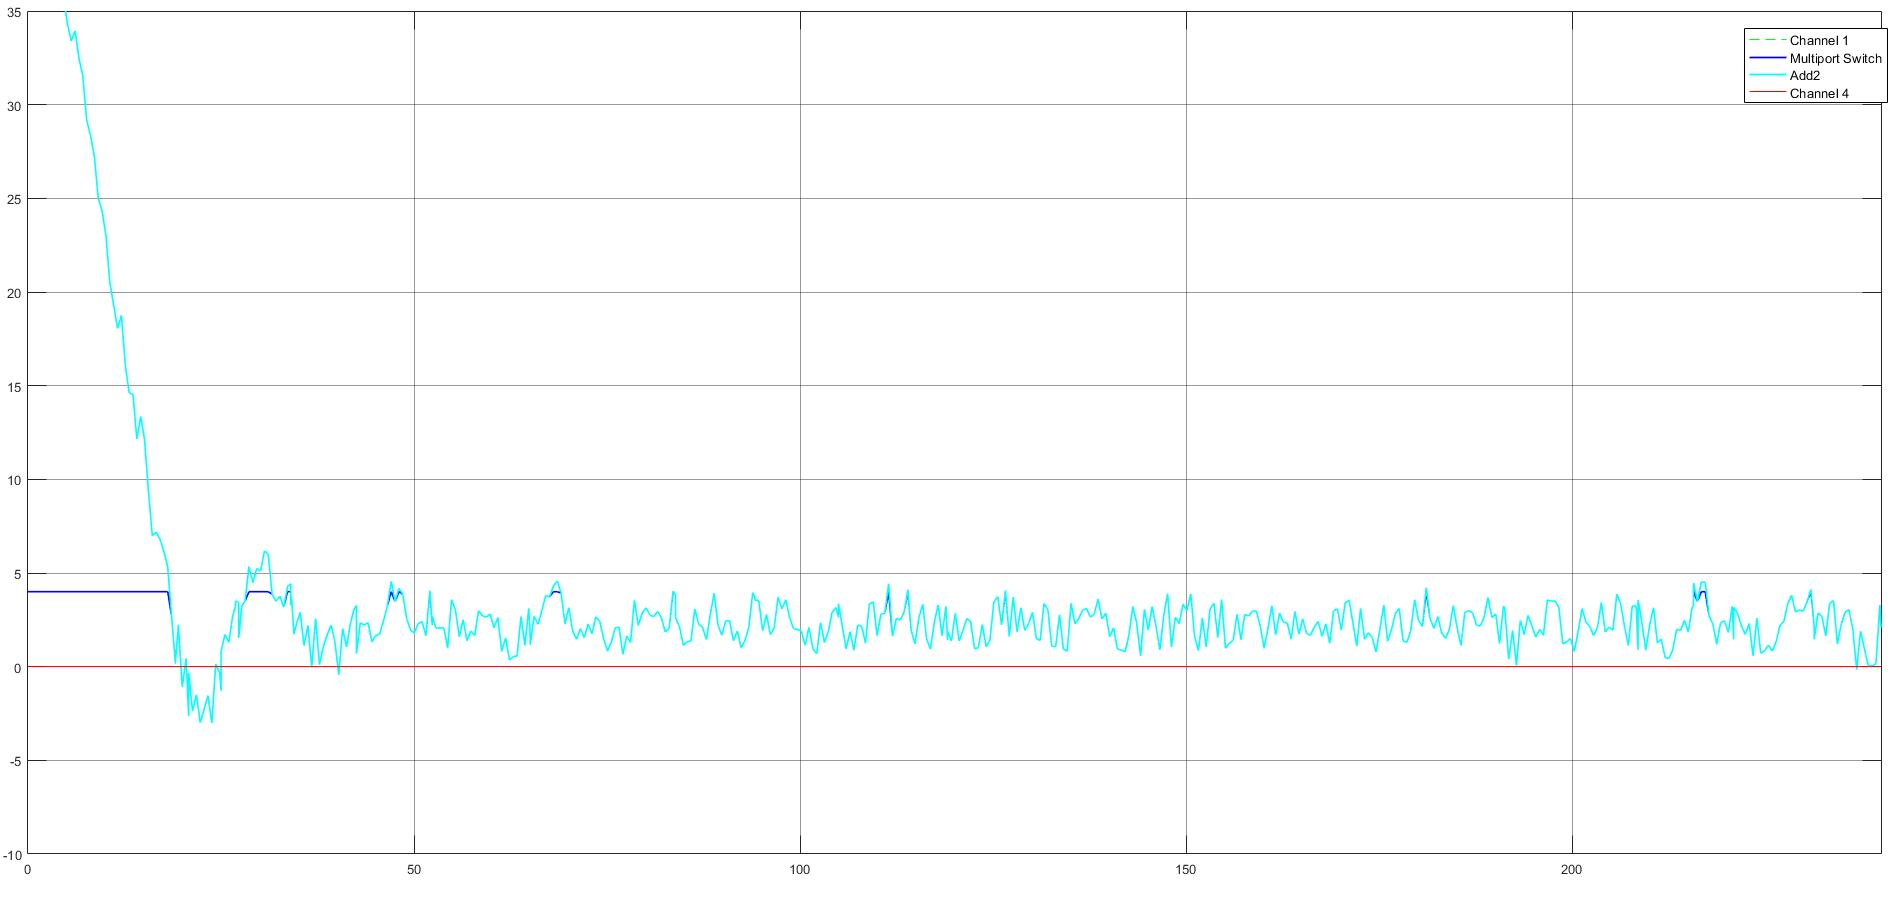
\includegraphics[scale=0.25]{9 - pi_11_segunda_ordem.jpg}
	\caption{Sinal de controle PI - Sistema de Segunda Ordem}
\end{figure}
\clearpage
\subsection{Implementação do controlador PID em segunda ordem}

O controlador PID reúne todas as ações vistas (proporcional, integral e derivativa), elas atuam no regime transitório e permanente. Utilizando os valores $K_p=7,5$, $K_i=0,015$ e $K_d=0,001$, diminuímos o \textit{overshoot}, mas não reduzimos a oscilação. O gráfico da saturação apresenta dois picos que chamam a atenção e não conseguimos consertar.

\begin{figure}[h]
	\centering
	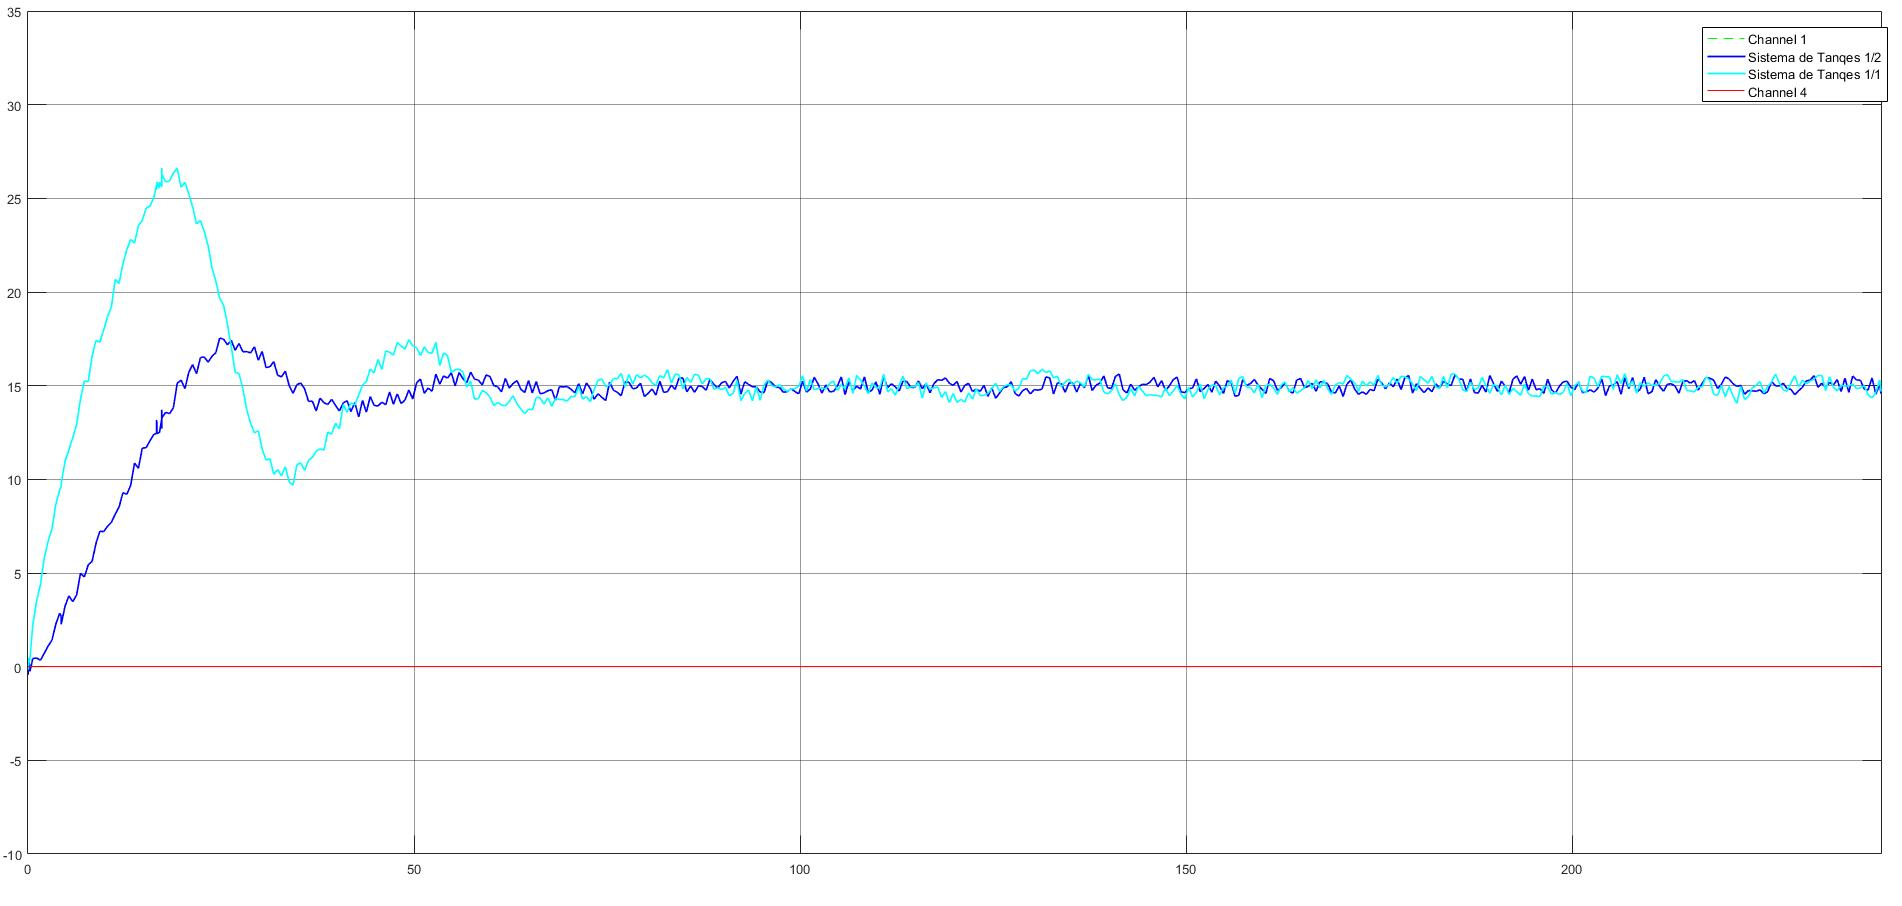
\includegraphics[scale=0.25]{10 - pid_1_segunda_ordem.jpg}
	\caption{Controlador PID - Sistema de Segunda Ordem}
\end{figure}

\begin{figure}[h]
	\centering
	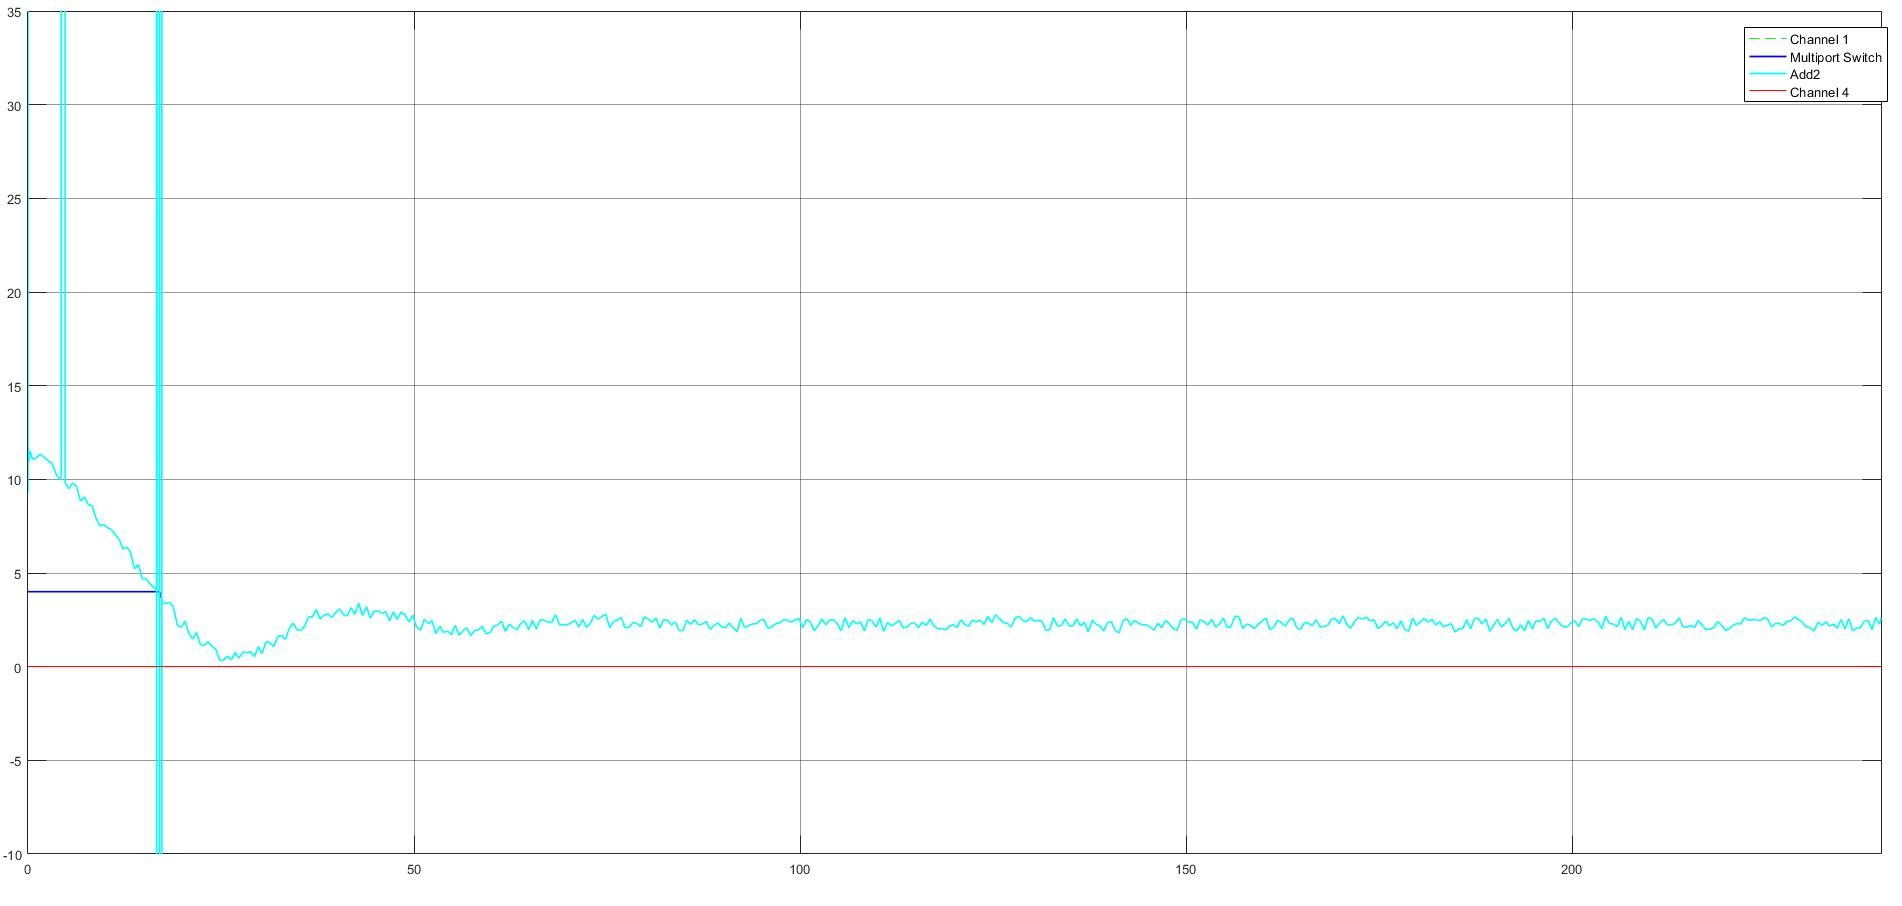
\includegraphics[scale=0.25]{10 - pid_11_segunda_ordem.jpg}
	\caption{Sinal de controle PID - Sistema de Segunda Ordem}
\end{figure}

Com esses valores o erro de regime não foi zerado, mas converge para o \textit{setpoint}.

\subsection{Implementação do controlador PID em segunda ordem com filtro derivativo}

A combinação de controlador PID com o filtro derivativo foi a que rendeu os melhores resultados, diferentemente desse conjunto aplicado ao sistema de primeira ordem, o sistema de segunda ordem se comportou muito melhor, diminuindo o erro de regime e o sobressinal.

\begin{figure}[h]
	\centering
	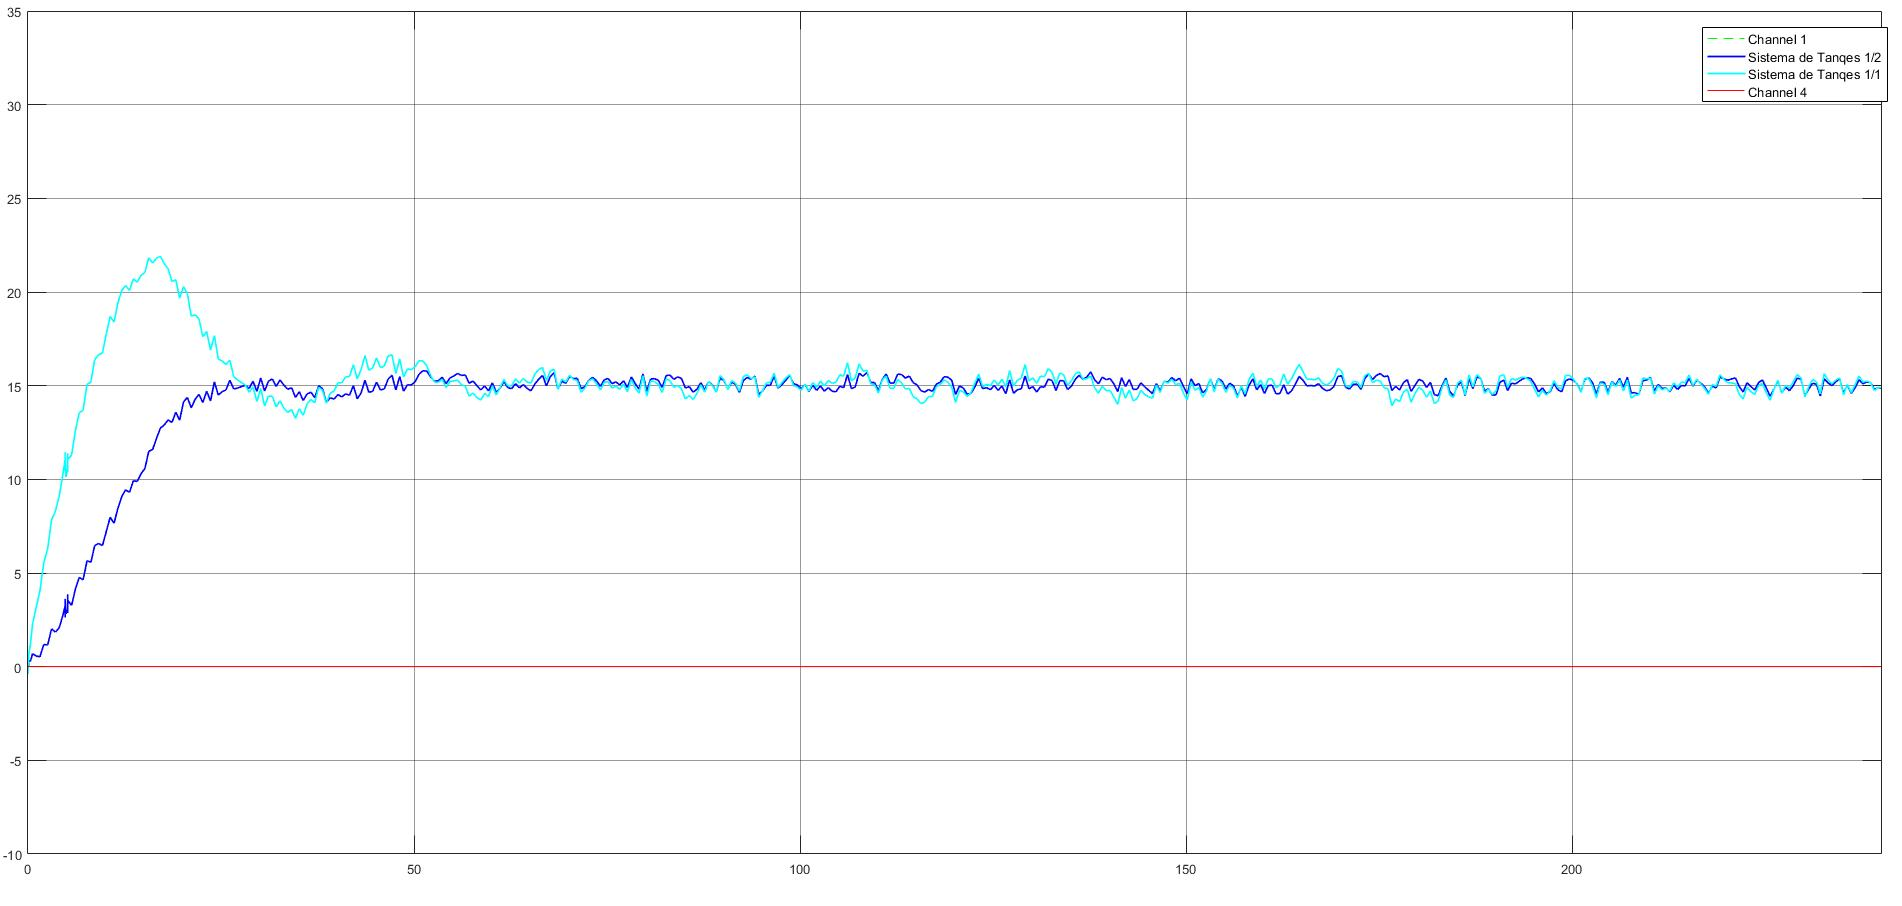
\includegraphics[scale=0.25]{12 - pid_segunda_ordem_filtro.jpg}
	\caption{Sinal de controle PID com filtro derivativo - Sistema de Segunda Ordem}
\end{figure}

No filtro \textit{anti-reset windup} usamos 0.01, já para as ações usamos $K_p=2,5$, $K_i=0,025$ e $K_d = 0,01$, curiosamente o valor usado no filtro e usado no $K_d$ é o mesmo, e dessa forma conseguimos o gráfico mostrado, mas não entendemos essa relação em específico. Foi notado, de forma empírica, que quando eles eram diferentes haviam mudanças mais significativas no gráfico. 
\phantompart

\section{Controle em cascata}

Na última parte do segundo experimento usamos dois controladores, sempre com o objetivo de melhorar o desempenho do sistema.

\subsection{Controlador PID com filtro derivativo }

O primeiro teste com o controlador em cascata foi usando um filtro derivativo nos dois controladores, nesse experimento foi utilizado um $K_{pe} = 2,5$. Nessa configuração obtemos um controlador que não era muito preciso em relação ao segundo tanque por causa do sobressinal, no primeiro reservatório o controle foi satisfatório, porque não havia \textit{overshoot} e o tempo de acomodação foi semelhante ao do segundo tanque.

\begin{figure}[h]
	\centering
	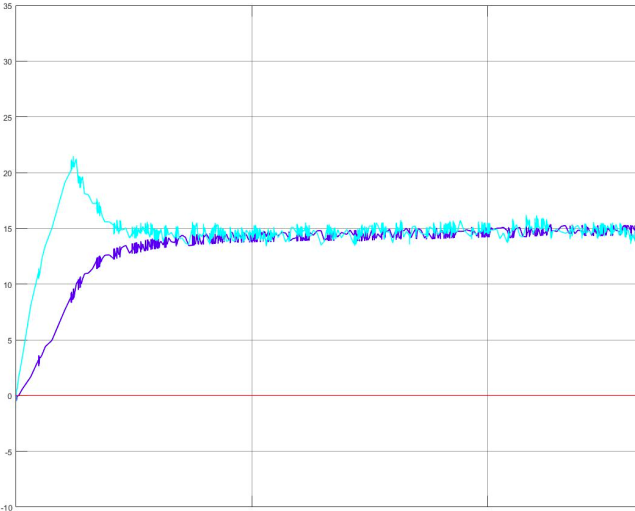
\includegraphics[scale=0.50]{13_cascata_1.png}
	\caption{Controlador PID em cascata - filtro derivativo}
\end{figure}

\subsection{Controlador PID com filtro derivativo e \textit{anti-reset windup}}

Nessa configuração começamos com $K_p = 2$, $K_i = 0,06$ e $K_d = 0.003$ para o mestre, e  $K_p = 1$, $K_i = 0,03$ e $K_d = 0.001$ para o escravo. Esses valores resultaram em uma anulação do \textit{overshoot} e uma convergência do sistema ao nível desejado, apesar disso, o sinal da malha mestre apresenta bastante ruído. Realizamos mais alguns testes, para tentar melhorar o comportamento apresentado pelo gráfico \ref{fig:controlador_cascata_2}, e assim obtivemos o gráfico \ref{fig:controlador_cascata_3}.

\begin{figure}[h]
	\centering
	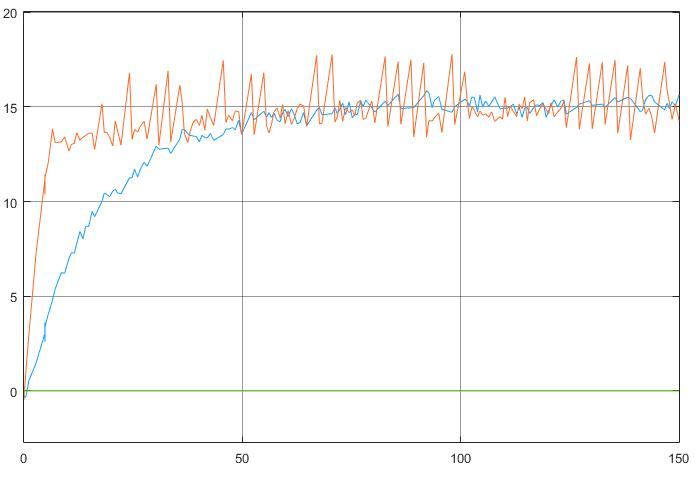
\includegraphics[scale=0.40]{14_controle_cascata_2.jpg}
	\caption{Controlador PID em cascata - filtro \textit{anti-reset windup}}
	\label{fig:controlador_cascata_2}
\end{figure}

\begin{figure}[h]
	\centering
	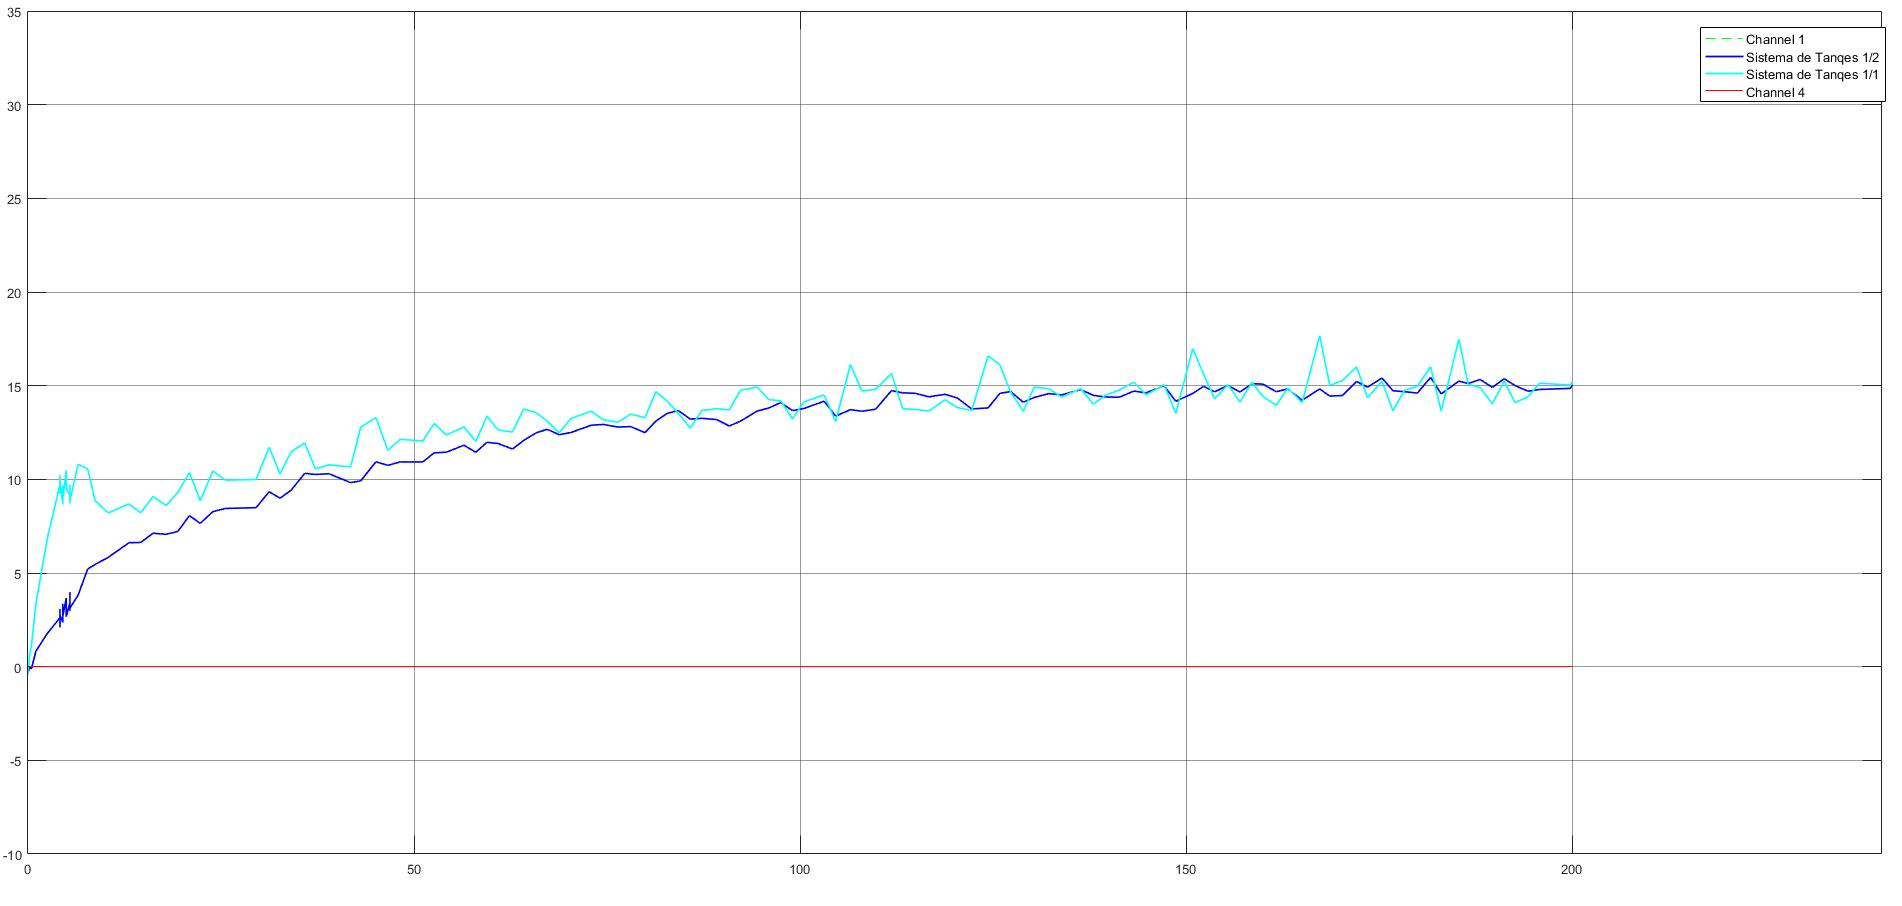
\includegraphics[scale=0.25]{15_controle_cascata_3.jpg}
	\caption{Controlador PID em cascata 2 - filtro \textit{anti-reset windup}}
	\label{fig:controlador_cascata_3}
\end{figure}

\chapter{Conclusão}

As simulações permitiram que fosse melhor entendido o comportamento dos controladores P, PI, PD e PID, e além desses, também implementamos os filtros, para entender o impacto que eles causam nos sinais dos controladores. Nos experimentos 2A e 2B o objetivo era controlar os níveis dos tanques 1 e 2, respectivamente, e no experimento 2C era pedido que apenas o segundo tanque fosse controlado. Para analisar os gráficos observamos o tempo de estabilidade, o tempo de subida, o sobressinal e a oscilação.

Foi observado que no sistema de primeira ordem, de acordo com nossas simulações, o tempo de estabilidade é menor em relação ao de segunda ordem, e também oscila menos. Além disso, esperávamos encontrar resultados melhores com o controle em cascata, porém o tempo de estabilidade aumentou e também ficou mais instável, isso pode ser um problema de \textit{tunning}, mas mesmo com pesquisa e vários testes empíricos não chegamos a um resultado realmente bom, que justifique o aumento de complexidade na implementação do controle em cascata numa planta industrial real, por exemplo.

Em todos os experimentos foi possível ver a ação proporcional, integral e derivativa, e as consequências de cada uma delas nos gráficos. Portanto, para diminuição de erro de regime, regula-se o $K_i$, para atuar na oscilação usamos o $K_p$ e para tornar o tempo de acomodação menor é importante usar o $K_d$.


\postextual

% ----------------------------------------------------------
% Referências bibliográficas
% ----------------------------------------------------------
\bibliography{abntex2-modelo-references}

\phantompart

\printindex

\end{document}
